\documentclass[12pt, floatsintext, man]{apa6}

\usepackage{amssymb}
\usepackage{graphicx}
\usepackage[outdir=./]{epstopdf}
%\DeclareGraphicsExtensions{.eps}

\usepackage{enumerate}
\usepackage{apacite}
\usepackage{listings}
\usepackage{multirow}

\newenvironment{figurehere}
	{\def\@captype{figure}}
	{}

\usepackage{lipsum}
%\pagenumbering{gobble}
%\usepackage{apacite}

\linespread{1.5}
\usepackage{textcomp}

\DeclareGraphicsRule{.tif}{png}{.png}{`convert #1 `dirname #1`/`basename #1 .tif`.png}
  
\makeatother

\title{Why do you ask? Good questions provoke informative answers.}
\shorttitle{Dots}
\author{Robert X.D. Hawkins, Noah D. Goodman}
\affiliation{Stanford University}

\abstract{What makes a question useful? What makes an answer appropriate? In this paper, we formulate a family of increasingly  sophisticated models of question-answer behavior within the Rational Speech Act framework. We compare these models based on three different pieces of evidence: first, we demonstrate how our answerer models capture a battery of four classic effects in psycholinguistics, which show that an answerer's level of informativeness varies with the inferred questioner goal. Second, we jointly test the questioner and answerer components of our model based on empirical evidence from a simple question-answer reasoning game. Third, we designed a real-time, multi-player version of this game with a wider range of conditions, which allows us to distinguish among the questioner models. We find that sophisticated pragmatic reasoning is needed to account for some critical aspects of the data. People can use questions to provide cues to the answerer about their interest, and can select answers that are informative about inferred interests.
}

\keywords{pragmatics, computational modeling}

\authornote{This research took place while the first author was a student at Indiana University. He is now at Stanford University, Stanford, CA 94305, USA. This work was supported by National Institute of Mental Health Grant 05771710 awarded to J. T. T. We thank Devin Burns for helpful comments on the experiment reported, and Patricia Knapp for her assistance in data collection. Correspondence concerning this article should be addressed to Robert X.D. Hawkins, e-mail: rxdh@stanford.edu}

\begin{document}
\maketitle
\section{Introduction}

\begin{quote}
Q:``Are you gonna eat that apple?''\\ A:``Oh, go ahead!''
\end{quote}

In this exchange, Q wants to know whether she can eat A's apple. Instead of directly asking this question, Q strategically chooses a question that differs from her true interest, avoiding an impolite question, yet still manages to send a signal to A about her true intentions. A, in turn, reasons beyond the overt question and provides an answer that addresses Q's true interests. This subtle interplay highlights the prevalence of social reasoning tasks in everyday dialogue and raises two specific questions for formal models of language:
What makes a question useful? And what makes an answer appropriate? 

A number of psycholinguistic studies have provided evidence that answerers are both sensitive to a questioner's goals and attempt to be informative with respect to those goals.
For instance, in the classic study of \citeA{Clark79_IndirectSpeechActs}, researchers called liquor merchants and opened the conversation with one of two sentences to set context: ``I want to buy some bourbon'' (the \emph{uninformative} condition) or ``I've got \$5 to spend'' (the \emph{five dollar} condition). They then asked, ``Does a fifth of Jim Beam cost more than \$5?'' Merchants gave a literal yes/no answer significantly more often in the latter condition than the former, where an exact price was more common. When provided with the five dollar context, the merchant inferred that the questioner's goal was literally to find out whether or not they could afford the whiskey, hence a simple `yes'  sufficed. In the uninformative context, however, the merchant inferred that the questioner's goal was just to buy whiskey, so the exact price was the most relevant response \cite{Clark79_IndirectSpeechActs}. 

Context and questioner goals have also been implicated in accounts of answers to identification questions like ``who is X?'' \cite{BoerLycan75_KnowingWho}, questions like ``Do you have the time?'' that permit answers with different degrees of approximation to the true value \cite{DerHenstCarlesSperber02_RelevanceTellingTime, GibbsBryant08_OptimalRelevance}, and to questions like ``where are you?'' that permit answers at many levels of abstraction \cite{Potts12_CardsDialogueCorpus}. While most of this work has focused on \emph{answerer} behavior, it suggests that the question itself is important in prompting a relevant answer.

%
%Since both questioners and answerers appear to be acutely sensitive to one another's intentions and knowledge, what makes a question useful? What makes an answer to a question useful? In this paper, we present three progressively more sophisticated computational models of question-answer behavior, which formalize and probe this deep interaction between the way answerers infer intentions and the way questioners signal them. We compare these models on the basis of two simulations of classic question-answer phenomena and one experiment in which participants must ask and answer questions given a fixed set of goals. We find that a sophisticated pragmatic answerer is needed to account for the data, and close by proposing that the purpose of questions in dialogue is to provide cues to the answerer about the questioner's goals and intentions.

%A number of studies in psycholinguistics have provided evidence that answerers are both sensitive to a questioner's goals and attempt to be informative with respect to those goals. For example, when people are asked `Do you have the time?'' they typically round their answers to the nearest 5 or 10 minute interval, even when they're wearing a digital watch \cite{DerHenstCarlesSperber02_RelevanceTellingTime}. However, if the question is preceded by the statement ``My watch stopped,'' people make their response precise to the minute  \cite{GibbsBryant08_OptimalRelevance}. While an approximate time is sufficiently informative with respect to most goals, like making it to a meeting on time, this experiment demonstrated that answerers were able to infer that the goal of setting a watch required more precise information.

Recent work on Rational Speech Act (RSA) models \cite{FrankGoodman12_PragmaticReasoningLanguageGames, GoodmanStuhlmuller13_KnowledgeImplicature} has mathematically formalized pragmatic language understanding as a form of recursive Bayesian inference, where listeners reason about speakers who choose utterances that maximize information gained by an imagined listener.
%a particular utility function (dependent on the listener's expected information gain). 
In this paper we extend the RSA framework to address simple question-answer dialogs.
%asking questions and giving answerers. 
The immediate challenge in doing so is that the speaker utility in RSA is based on direct information provided by an utterance---since questions don't provide direct information, we must say what utility they do have. 

We suggest, following \citeA{VanRooy03_QuestioningDecisionProblems}, that the value of a question is the extent to which it can be expected to elicit information relevant to the questioner later in the dialogue. 
More specifically, for the questioner, the value of a question is the expected information gained about her interests, given the set of likely answers it may provoke. 
This diverges from regular RSA in that the value of a question depends on information gained by the speaker (rather than listener), and that this information comes later in the (very short) conversation.

To fully specify this questioner we need a model of the answerer, which can serve as both the model assumed by a questioner, and as a model of answer behavior itself. We explore three, increasingly sophisticated, answerer models. The simplest answerer provides a literal answer to the question (without attempting to be informative);   
the explicit answerer attempts to be informative with respect to the explicit question asked (without inferring the questioner's underlying interests);  
the pragmatic answerer infers the most likely true interests of the questioner, and then informatively addresses those interests.
The latter model extends RSA to reason about the topic of conversation, as proposed by \citeA{KaoWuBergenGoodman14_NonliteralNumberWords} to explain hyperbole; it goes beyond previous work by using the explicit question as a (potentially indirect) cue to this topic. 

%In particular, we compare a pragmatic answerer making inferences about the questioner's goals to two simpler models: one that takes into account only that an answerer wants to be maximally informative with respect to the explicit question asked (without inferring the questioner's underlying decision problem) and one that provides a literal answer to the question (without attempting to be maximally informative).  


%% I think we need to discuss at least one previous model, to make it clear why the problem we're tackling is a problem in the first place. The rest can be in related work at the end.
%Recent formal models of question-answer pragmatics have made progress by formally specifying the questioner's goals and what it means for an answerer to be informative with respect to them. van Rooy \citeyear{VanRooy03_QuestioningDecisionProblems}, for instance, defines a goal as a utility function defining a decision problem faced by the questioner. A useful answer under this decision theoretic account is one that maximizes the expected value of the questioner's utility by reducing their uncertainty about the true state of the world. A useful question is one that allows for a sufficiently fine-grained set of answers, optimally distinguishing the worlds relevant to their decision problem. While this framework elegantly accounts for the context-dependence and relevance-maximization of question and answer behavior, it assumes that the questioner's decision problem is known \emph{a priori} by the answerer or fully determined by context. This minimizes the role of the questioner; they just establish a space of answers and then let the answerer do the rest of the work. If the answerer is so adept at using context to determine the relevant information, though, why does the questioner need to ask a question in the first place? Is it just a formality, to prompt the other for their information, or does it serve as a signal in itself, as the studies above suggest? 
%
%We claim that the questioner must reason about answerer behavior, in order to determine what question will produce the most useful answers. This raises a further issue: what kind of answerer does the questioner reason about, and is this internal model accurate? 

The rest of this paper is structured as follows. First, we lay out the details of our computational questioner and answer models.
%we specify a family of questioner and answerer agents, highlighting some points of divergence from previous RSA models. 
%We then formally individuate literal, explicit, and pragmatic models in this family, which represent different hypotheses about how questioners and answerers reason about their task. 
%In particular, we compare a pragmatic answerer making inferences about the questioner's goals to two simpler models: one that takes into account only that an answerer wants to be maximally informative with respect to the explicit question asked (without inferring the questioner's underlying decision problem) and one that provides a literal answer to the question (without attempting to be maximally informative).  
We then present a set of computational experiments demonstrating how this set of models captures four classic answerer-sensitivity effects from the psycholinguistics literature. Because data on \emph{questioner} behavior is relatively sparse, we collected data in a simple communication game paradigm allowing us to manipulate private goals, potential questions, and potential answers. After testing the predictions of the different models on data from a simple single-player version of the task, we scale up this paradigm to a more natural real-time, multi-player experiment using a wider variety of goal sets, question sets, and answer sets. We dedicate particular attention to one condition in which the questioners models make different predictions.
%We find that the most sophisticated, pragmatic models best account for human performance.
%derive predictions for a  of experiments using a novel guessing-game task, and compare these predictions to human performance. 
%In one phase of the task, we require participants to ask a question (from a fixed set of possible questions), given a decision problem. In the second phase, we require participants to give an answer (from a fixed set of possible answers) to a question (from a fixed set of possible questions). 
We close with a brief discussion of related models and future directions.
%These models and data, combined with the psycholinguistic data above, seeks to place question-answer behavior in the larger class of social behavior governed by theory of mind.

\section{A Rational Speech Act model of question and answer behavior}
\label{sec:model}

How should a questioner choose between questions?
%
We start by assuming that the questioner aims to \emph{learn information relevant to a private goal}.
%
In order to choose a question that results in useful information, the questioner reasons about how the answerer would respond, given different possible states of the world; she selects a question that results in an answer that tends to provide goal-relevant information.
%

% This is a divergence from previous RSA models, where agents choose utterances with the goal of imparting information about the state of the world.

More formally, suppose there is a set of world states $\mathcal{W}$, a set of possible goals $\mathcal{G}$, a set of possible questions $\mathcal{Q}$, and a set of possible answers $\mathcal{A}$.
These sets are taken to be in common ground between the questioner and the answerer.
An informational goal $g \in \mathcal{G}$ is a projection function that maps a world state to a particular feature or set of features that the questioner cares about; this is similar to the notion of a question-under-discussion \cite{Roberts96_InformationStructureDiscourse}.
We will use the notation $P_{g}(w)$ to indicate the probability $\hat{P}(g(w))$ of the $g$-relevant aspect of $w$ under the projected distribution 
$\hat{P}(v) = \int_{\mathcal{W}} \delta_{v=g(w)}P(w)dw$.
% Each of these projections corresponds to a different utility function, in a decision-theoretic formulation.
%In order to learn information about their private goal $g$, the questioner reasons about how an internal model of an answerer would respond given some true world.

\newcommand{\KL}[2]{\ensuremath{D_{KL}({#1}\, \| \, {#2})}}
\newcommand{\E}[2]{\ensuremath{\mathbb{E}_{#1}\left [#2 \right]}}

The \textbf{questioner} takes a goal $g \in \mathcal{G}$ as input and returns a distribution over questions $q \in \mathcal{Q}$:
%
$$ 
P(q|g) \propto e^{\E{P(w^*)}{\KL{P_g(w|q, w^*)}{P_g(w)}} - C(q)} 
$$
%
It trades off the cost of asking a question, $C(q)$, and expected information gain. The cost likely depends on question length, among other factors. Information gain is measured as the Kullback-Leibler divergence between the prior distribution over $g$-relevant worlds, $P_g(w)$, and the posterior distribution one would expect after asking a question $q$ whose answer reflected true world state $w^*$:
%
$$ P_g(w|q, w^*) = \sum_{a \in \mathcal{A}} P_g(w |q, a) P(a| q, w^*)$$
%
%This conditional distribution reflects the fact that the answerer (who knows the true world state $w$) may behave noisily, have a limited set of possible answers, or other limitations.
%to questioner (who is inferring a world state $w^*$) is affected by stochastic answerer behavior and a limited set of possible answers. 
This distribution has two components: 
First, it depends on $P(a | q, w^*)$, a model of the answerer which we will explore shortly.
Second, it depends on (the goal projection of) $P(w | q, a)$, an `interpreter' that specifies the likelihood assigned to different worlds given question and answer pairs.

To define the interpreter function, which all agents use to compute the literal interpretation of a question-answer pair, we must assign questions a semantic meaning.
We assume that a question is an informational goal that projects from worlds to the answer set $\mathcal{A}$.
This is equivalent to the more common partition semantics of \citeA{GroenendijkStokhof84_SemanticsOfQuestions}, as can be seen by considering the pre-image of such a projection; an answer picks out an element of the partition via $q^{-1}(a)$.
% \red{JD: how can we see this, exactly?} \red{RDH: we say this in the next sentence, right? $q^{-1}(a)$ gives the cell of the partition corresponding to the given aspect of interest\dots}
%An answer-value (as opposed to the answer utterance) is a possible value of the projection function (which picks out an element of the partition via $q^{-1}(a)$).
%The explicit question can be assigned a literal meaning which is a projection from worlds to answer values (this is equivalent to the common partition semantics of questions \cite{gronendijk}).
% likelihood of a world given a question and an answer.
%For the purposes of this paper, we will use Groenendijk \& Stokhof semantics \citeyear{GroenendijkStokhof84_SemanticsOfQuestions}, where a question induces a partition $\mathcal{P}_q$ over the space of possible world and each cell of this partition is an equivalence class corresponding to a different answer. An answer, then, selects a cell of this partition, denoted by $\mathcal{P}_q(a)$, which is a set.
The \textbf{interpreter} constrains the prior on worlds to the subset of its support that is consistent with the semantics of a question-answer pair\footnote{We should also have a semantic evaluation function that maps an answer utterance to its value in $\mathcal{A}$. For clarity we assume this is a trivial mapping and suppress it.}:
%
$$P(w | q, a) \propto P(w) \delta_{q(w)=a}$$



We next describe three different answerer models; the questioner could assume any one of them, leading to three corresponding versions of the questioner model.
All answerers take a question $q \in \mathcal{Q}$ and a true world state $w^* \in \mathcal{W}$ as input and return a distribution over answers $a \in \mathcal{A}$.
%
The \textbf{literal answerer} simply chooses answers by trading off prior answer probability  and how well a question-answer pair conveys the true state of the world to an interpreter:
%
$$P(a | q,w^*) \propto P(a) P(w^* | q, a) $$
%
For a fixed question, this is equivalent to the speaker in previous RSA models. The question enters only in specifying the literal meaning of an answer.
%
The \textbf{explicit answerer} additionally evaluates answers with respect to how well they address the explicit question $q$:
%
$$P(a | q, w^*) \propto P(a) P_q(w^* | q, a) $$

The \textbf{pragmatic answerer} also evaluates answers with respect to how well they address the informational goal, but doesn't take the question's explicit meaning at face value. Instead, the pragmatic answerer reasons about which goals $g$ are likely given that a question $q$ was asked, and chooses answers that are good on average:
%% FIXME: restrict to truthful answers
%
$$
P(a | q, w^*) \propto p(a) \sum_{g \in \mathcal{G}} P(g|q) P_g(w^*|q, a)
$$
Reasoning backwards from questions to goals is a simple Bayesian inversion of the (explicit) questioner using a prior on goals:
$$
P(g|q) \propto P(q|g)P(g)
$$

For all of the questioner and answerer models, we can vary how strongly optimizing they are---that is, to what extent they are sampling from the distributions defined above, and to what extent they deterministically choose the most likely element. For any such distribution over utterances, we introduce an optimality parameter $\alpha$ and transform it by $ P'(x) \propto P(x)^{\alpha} $.
%

This concludes our specification of the model space, giving a set of three answerers and three corresponding questioners that reason about them. We have implemented these models in WebPPL, a probabilistic programming language \cite{GoodmanStuhlmuller14_DIPPL}, and runnable code for all reported simulations will be available online at \url{http:// hawkrobe.github.io/Q\_and\_A/}. The model predictions shown throughout the rest of the paper are computed using this implementation. 

\subsection{Related models}

The above probabilistic model of question and answer behavior bears some resemblance to recent decision theoretic \cite{VogelBodoiaPottsJurafsky13_GricePOMDP} and game theoretic \cite{Franke13_GameTheoryPragmatics} models of pragmatic reasoning. In particular, all these approaches emphasize \emph{reasoning} and \emph{inference} about a partner's underlying mental state. In this respect, these theories contrast with the popular interactive alignment model \cite{PickeringGarrod04_BBS_Dialogue} and other dynamical systems models of dialogue \cite<e.g.>{FusaroliTylen15_Synergy},  where coordination occurs through a process of priming and adjusting to a partner's syntactic, lexical, and phonological choices. 

While there is a growing literature on dialogue models in general, far less attention has been devoted to the specifics of question and answer dynamics. The primary theoretical work in this area derives from formal linguistic theories, which focused on the notion of informativeness. In Groenendijk and Stokhof's\citeyear{GroenendijkStokhof84_SemanticsOfQuestions} foundational work on question and answer semantics, asking a question induces a partition over the space of possible worlds, where each cell of the partition corresponds to a possible answer. An answer, then, consists of eliminating cells in this partition, and the most useful answers are those that eliminate all relevant alternatives to the true world. However, as van Rooy \citeyear{VanRooy03_QuestioningDecisionProblems} and others \cite{Ginzburg95_ResolvingQuestions} have pointed out, this predicts that wh-questions like ``Where can I buy an Italian newspaper?'' can only be fully resolved by exhaustively mentioning whether or not such a newspaper can be bought at each possible location. Clearly, this is not the case: a single nearby location would suffice. These theories also cannot account for contextual variation in what counts as a useful answer.

More recent theories have tried to fix these problems by introducing some consideration of the questioner's goals. \citeA{VanRooy03_QuestioningDecisionProblems}, for instance, formalizes these goals as a decision problem faced by the questioner. A useful answer under this decision theoretic account is one that maximizes the expected value of the questioner's decision problem. A useful question is one that induces a sufficiently fine-grained partition, optimally distinguishing the worlds relevant to the decision problem. While this framework elegantly accounts for the context-dependence and relevance-maximization of question and answer behavior, it assumes that the questioner's decision problem is known a priori by the answerer. If this were the case, the act of asking questions would seem irrelevant: why wouldn't the answerer directly tell the questioner which action to take? Nevertheless, while empirical work has almost exclusively focused on answerer behavior, van Rooy's approach suggests that the question itself is important in prompting a relevant answer. 

Our models are an effort to expand on this core idea in a probabilistic framework that also provides an inferential mechanism for the answerer to infer the `decision problem' instead of assuming it. We now proceed to show how these models address four classic examples of question and answer pragmatics from the psycholinguistics literature.

\section{Four case studies}

\subsection{Clark (1979), Experiment 4}

First, we show that our model can provide different---sometimes over- or under-informative---answers to the same explicit question, depending on context. For this illustration, we model the whiskey-pricing study presented in the Introduction \cite{Clark79_IndirectSpeechActs}. Recall that liquor merchants were more likely to give over-informative answers (specifying exact price) to the question ``Does a fifth of Jim Beam cost more than \$5?'' in the uninformative context (``I want to buy some bourbon'') than in the five dollar context (``I've got \$5 to spend'').

Our world state is simply the whiskey's price (\$1, \$2, \dots, \$10). There are two possible goals: learning the price of whiskey and learning whether the price is greater than \$5. The set of answers includes exact prices as well as ``yes'' and ``no'', with lower cost for ``yes'' and ``no'' than the price statements. We model the context sentence as affecting the questioner's goal prior. When the context is ``I'd like to buy some whiskey,'' we assume that the the two goals are equally likely. When it is ``I only have \$5 to spend,'' we assume that it is 9:1 in favor of learning whether the price is greater than \$5.

\subsubsection{Results} When the question is ``Does Jim Beam cost more than \$5?'', the correct Boolean answer is  the most probable choice (at probability $.44$ and $.49$). Critically, there is a context-dependence for answers to this question: when prefaced with ``I'd like to buy some whiskey.'', the correct exact price answer is favored more strongly (at probability $.18$) than when the context is ``I only have \$5 to spend.'' (probability $.11$). By contrast, the literal and explicit answerers (which have no natural way to account for context) do not make differential predictions in the two situations. The literal model predicts that the answerer is equally likely to say the true Boolean answer and the true numerical answer, and the explicit model predicts that the answerer will always give the true Boolean answer, since it is the explicit question being asked. This suggests that our pragmatic \emph{answerer} is consistent with human behavior in psychologically interesting situations, passing a first, qualitative, test. 

\subsection{Groenendijk and Stokhof (1984)}

For a slightly more complex example, we consider the classic puzzle of \emph{mention-some} and \emph{mention-all} readings of wh-questions  \cite{GroenendijkStokhof84_SemanticsOfQuestions,SchulzVanRooij06_ExhaustiveInterpretation}. Some questions, like ``Who is coming to dinner tonight?'' are intended to elicit an exhaustive list of the entities that are answers. For other questions, like ``Where can I find a bathroom in this building?'', a single answer would be sufficient. 

The question ``Where can one buy an Italian newspaper?'' can intuitively be ambiguous between these meanings depending on who is asking: if it is a tourist, they probably just want to know the nearest place, but if it is a businessperson trying to build a newspaper distribution network in town, they likely want the whole list. The puzzle is determining how the same question can take on different semantics in different contexts: according to our account, this happens via an inference about the questioner's underlying goal.

Our world state is an object consisting of four cafes in town. Each cafe is assigned two properties: its distance from the speaker and whether or not it sells Italian newspapers. There are two possible goals: learning the identity of the \emph{nearest} cafe selling a newspaper and learning the identity of \emph{all} cafes selling a newspaper. The set of answers includes all 16 combinations of different cafes (e.g. ``cafe 1 and cafe 3'' or ``cafe 2, cafe 3, and cafe 4''), as well as the answer ``none''. 

The prior over answer utterances is constructed as follows: there is a 10\% chance of saying ``none,'' . Otherwise, the agent selects one of the four cafes and terminates with probability .5. If the agent does not terminate, they pick another cafe from the list and continue until either terminating or running out of possible cafes. This naturally gives longer answers lower probability, reflecting their higher cost of utterance. We model the context sentence as affecting the questioner's goal prior: if they say ``I'm new here,'' there is a 9:1 chance that they are interested in the closest location with a newspaper; if they say ``I'm a businessperson\dots,'' there is a 9:1 chance that they are interested in all of the newspaper locations. 

\subsubsection{Results}

For concreteness, we set the world to be the following :

\begin{lstlisting}
world = {'cafe1' : [3, false],
         'cafe2' : [1, true],
         'cafe3' : [3, true],
         'cafe4' : [3, true]}
\end{lstlisting}
and enumerated over all model executions for both contexts. We find that the highest probability response given the ``I'm new here'' context is the single location ``cafe2,'' with probability 0.56. Given the ``I'm a businessperson\dots'' context, however, the highest probability response is the conjunction ``cafe2 and cafe3 and cafe4,'' with probability 0.82. Note that cafe 1 was not assigned any probability in either context because it did not sell Italian newspapers (demonstrating that the pragmatic answerer will not lie), and that the nearest cafe was given precedence in the ``tourist'' context. 

The literal and explicit answerers, as in the Clark scenario, do not have the means of making inferences about the questioner's underlying goals. Thus, both models incorrectly predicted that the context would not affect the preferred response. The literal answerer predicted that all combinations of cafes 2, 3, and 4 would be given in proportion to their prior likelihood (with no special preference given to the closest one). The explicit answerer predicted that cafe2 would be preferred in all contexts.     Crucially, the only difference between our model of this scenario and the Clark scenario is the set of QUDs, the structure of the world, and the meanings of the answers. The questioner and answerer functions stayed exactly the same.

\subsection{Gibbs Jr. \& Bryant (2008): Experiment 3}

It has been shown in previous work that people typically round their answers to the nearest 5 or 10 minute interval when asked `Do you have the time?'', even when they're wearing a digital watch \cite{DerHenstCarlesSperber02_RelevanceTellingTime}.  \citeA{GibbsBryant08_OptimalRelevance} replicated this result, and then performed a follow-up study where they preceded their question by the context ``I have a meeting at 4:00.'' They found that the tendency to round times decreased as a function of the time remaining until the stated deadline: when people were asked at 3:40, they would say ``It's 3:45,'' but when people were asked at 3:53, they would make their response precise to the minute. They explain this result by appealing to the questioner's goals: while an approximate time is sufficiently informative with respect to most goals, a questioner who is running late to an appointment may have the goal of judging whether to rush, in which case a precise time is needed. 

We take the world state to be the true current time. Unlike in the previous two scenarios, where there are only two QUDs and two contexts that make each QUD more or less likely, we now let there be a \emph{family of QUDs} and a fixed context stating the time of the appointment. This family of QUDs is parameterized by a threshold time, below which times are rounded to the nearest 5 minute increment and above which times are given exactly. For example, the QUD with the threshold set at 3:50 corresponds to a goal of wanting to learn the true time if it is higher than 3:50 and only caring about the approximate time below 3:50. The prior over thresholds ($\tau =$ 3:30, 3:35, \dots, 3:55), given a context sentence, weights each threshold by its distance to the appointment time, reflecting the intuition that the questioner will be more interested in the exact time as it approaches the appointment time.

 The set of answers is the set of times that could be given (e.g. 3:30, 3:31, \dots, 4:00), with uniform probability. Critically, the meaning of an answer is not exact: it introduces a factor in the ``interpreter'' component of the model, upweighting world states that are close to the answer utterance. In other words, we specify an ``approximate'' semantics for number references, which is necessary for rounded answers to be produced in the first place.
 
 \subsubsection{Results}
 
 To test the behavior of this model, we compare two simulations. In both, the context is ``I have an appointment at 4:00.'' In the first, the true world state is 3:34 (the `appointment far' condition); in the second, the true world state is 3:54 (the `appointment near' condition). Gibbs Jr. and Bryant \citeyear{GibbsBryant08_OptimalRelevance} found that the answerer is most likely to round to 3:35 in the `appointment far' condition, but most likely to give the exact time, 3:54, in the `appointment near' condition. Indeed, in the `appointment far' condition, the pragmatic questioner model, which infers which threshold is likely given the context and threshold, replies the rounded time `3:35' with probability 0.40 compared to the true time `3:34' with probability 0.27. In the `appointment near' condition, this pattern reverses: the pragmatic questioner model replies the rounded time `3:55' with probability 0.16 and the exact time `3:54' with probability 0.68 (see Figure \ref{fig:timeExperimentResults}).
 
 \begin{figure}
\begin{center}
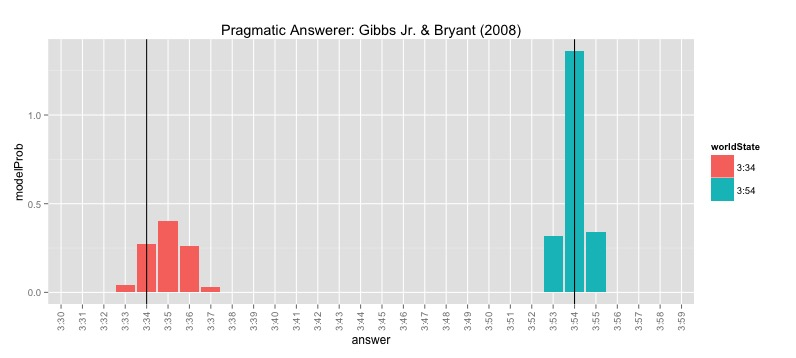
\includegraphics[scale = .5]{timeExpResults.jpeg}
\end{center}
\vspace{-.25cm}
\caption{Results for our computational experiments replicating Gibbs Jr. and Bryant (2008). Vertical lines represent the true world state.}
\label{fig:timeExperimentResults}
\end{figure}


\subsection{Clark (1979): Experiment 5}

Our final scenario is a critical test for the questioner component of our model: if our RSA model is correct, the questioner's choice of utterance itself should guide a pragmatic answerer's inferences about likely underlying goals. In a follow-up to the first experiment we modeled in this paper, \citeA{Clark79_IndirectSpeechActs} tested the inferences the merchant made about the questioner's goals on the basis of their question utterance, without hearing an explicit context sentence. The goal of the questioner was to find out all the kinds of credit cards the merchant accepted, and they could ask questions at different levels of specificity, e.g. ``Do you accept Master Charge cards?'' or ``Do you accept credit cards?'' or ``Do you accept any kinds of credit cards?'' He found that as the noun used in the question became less specific, literal \emph{yes/no} responses were less likely and the alternative (over-informative) response \emph{We accept x, y, z cards.} were preferred.

We have also not yet implemented this model, but the plan is to represent a world state as an object mapping each possible kind of credit card (Visa, Discover, MasterCard) to a boolean value representing whether the establishment will accept that card. There are four possible goals: learning whether or not the establishment accepts (1) Visa, (2) Discover, (3) MasterCard, or (4) learning the exact list of cards that the establishment accepts. The set of answers includes ``yes,'' ``no,'' and all possible lists of the three cards listed above, with ``yes'' and ``no'' slightly preferred for their lower cost. Because there is now a decision between different questions that the questioner must entertain, we must also specify a \emph{questioner} prior, which we set to uniform for simplicity. 

This suggests that our pragmatic \emph{answerer} is consistent with human behavior in psychologically interesting situations, passing a first, qualitative, test. However, we have not yet shown that the \emph{questioner} behavior matches that of humans. Indeed, the questioner has been largely neglected in studies of answering \cite<but see, e.g.,>{Potts12_CardsDialogueCorpus}, even though, as our opening example illustrates, the choice of question is important for understanding answers. In the next section we introduce an experimental paradigm that allows us to jointly explore quantitative behavior of both questioners and answerers. 

%\vspace{-1em}

\section{Exp.~1: Hierarchical questions and answers}

In order to simultaneously test how questioners choose questions when faced with a particular goal and how answerers respond  under uncertainty about this goal, we used a guessing-game task played by two players: a questioner and an answerer. In this game, $4$ animals (a dalmatian, a poodle, a cat, and a whale) were hidden behind $4$ gates. These animals corresponded to different levels in a class hierarchy (see Fig.~\ref{fig:taskhierarchy}). The questioner received a private goal of finding one of the objects (e.g. `find the poodle'), and the answerer (but not the questioner) knew the location of each object. Before choosing a gate, the questioner asked the answerer a single question, chosen from a restricted set of options, and the answerer responded by revealing the object behind a single gate. This restriction was motivated by one of the key features of our opening example: when the most direct question (``can I eat your food?'') is suppressed due to politeness, utterance length, complexity, or some other intervening factor, questioners must rely instead on an indirect question. 

This set of restricted options was critical to distinguishing between the pragmatic and explicit variants of our model. If all questions were equally available, both our `explicit' and `pragmatic' questioner models would prefer the most direct one. To see how they make different predictions in the presence of restrictions, suppose `poodle?' was not available the questioner. If the questioner asked about a `dog?', the poodle and dalmatian would be considered equally good options by an explicit answerer because they are both dogs. However, the pragmatic answerer could reason that if the questioner was truly interested in the location of the dalmatian, he would have \emph{asked} about the dalmatian. Because he didn't, he must be interested in the other valid response that he lacks a direct question for: the poodle. 

\begin{figure}[t!]
\begin{center}
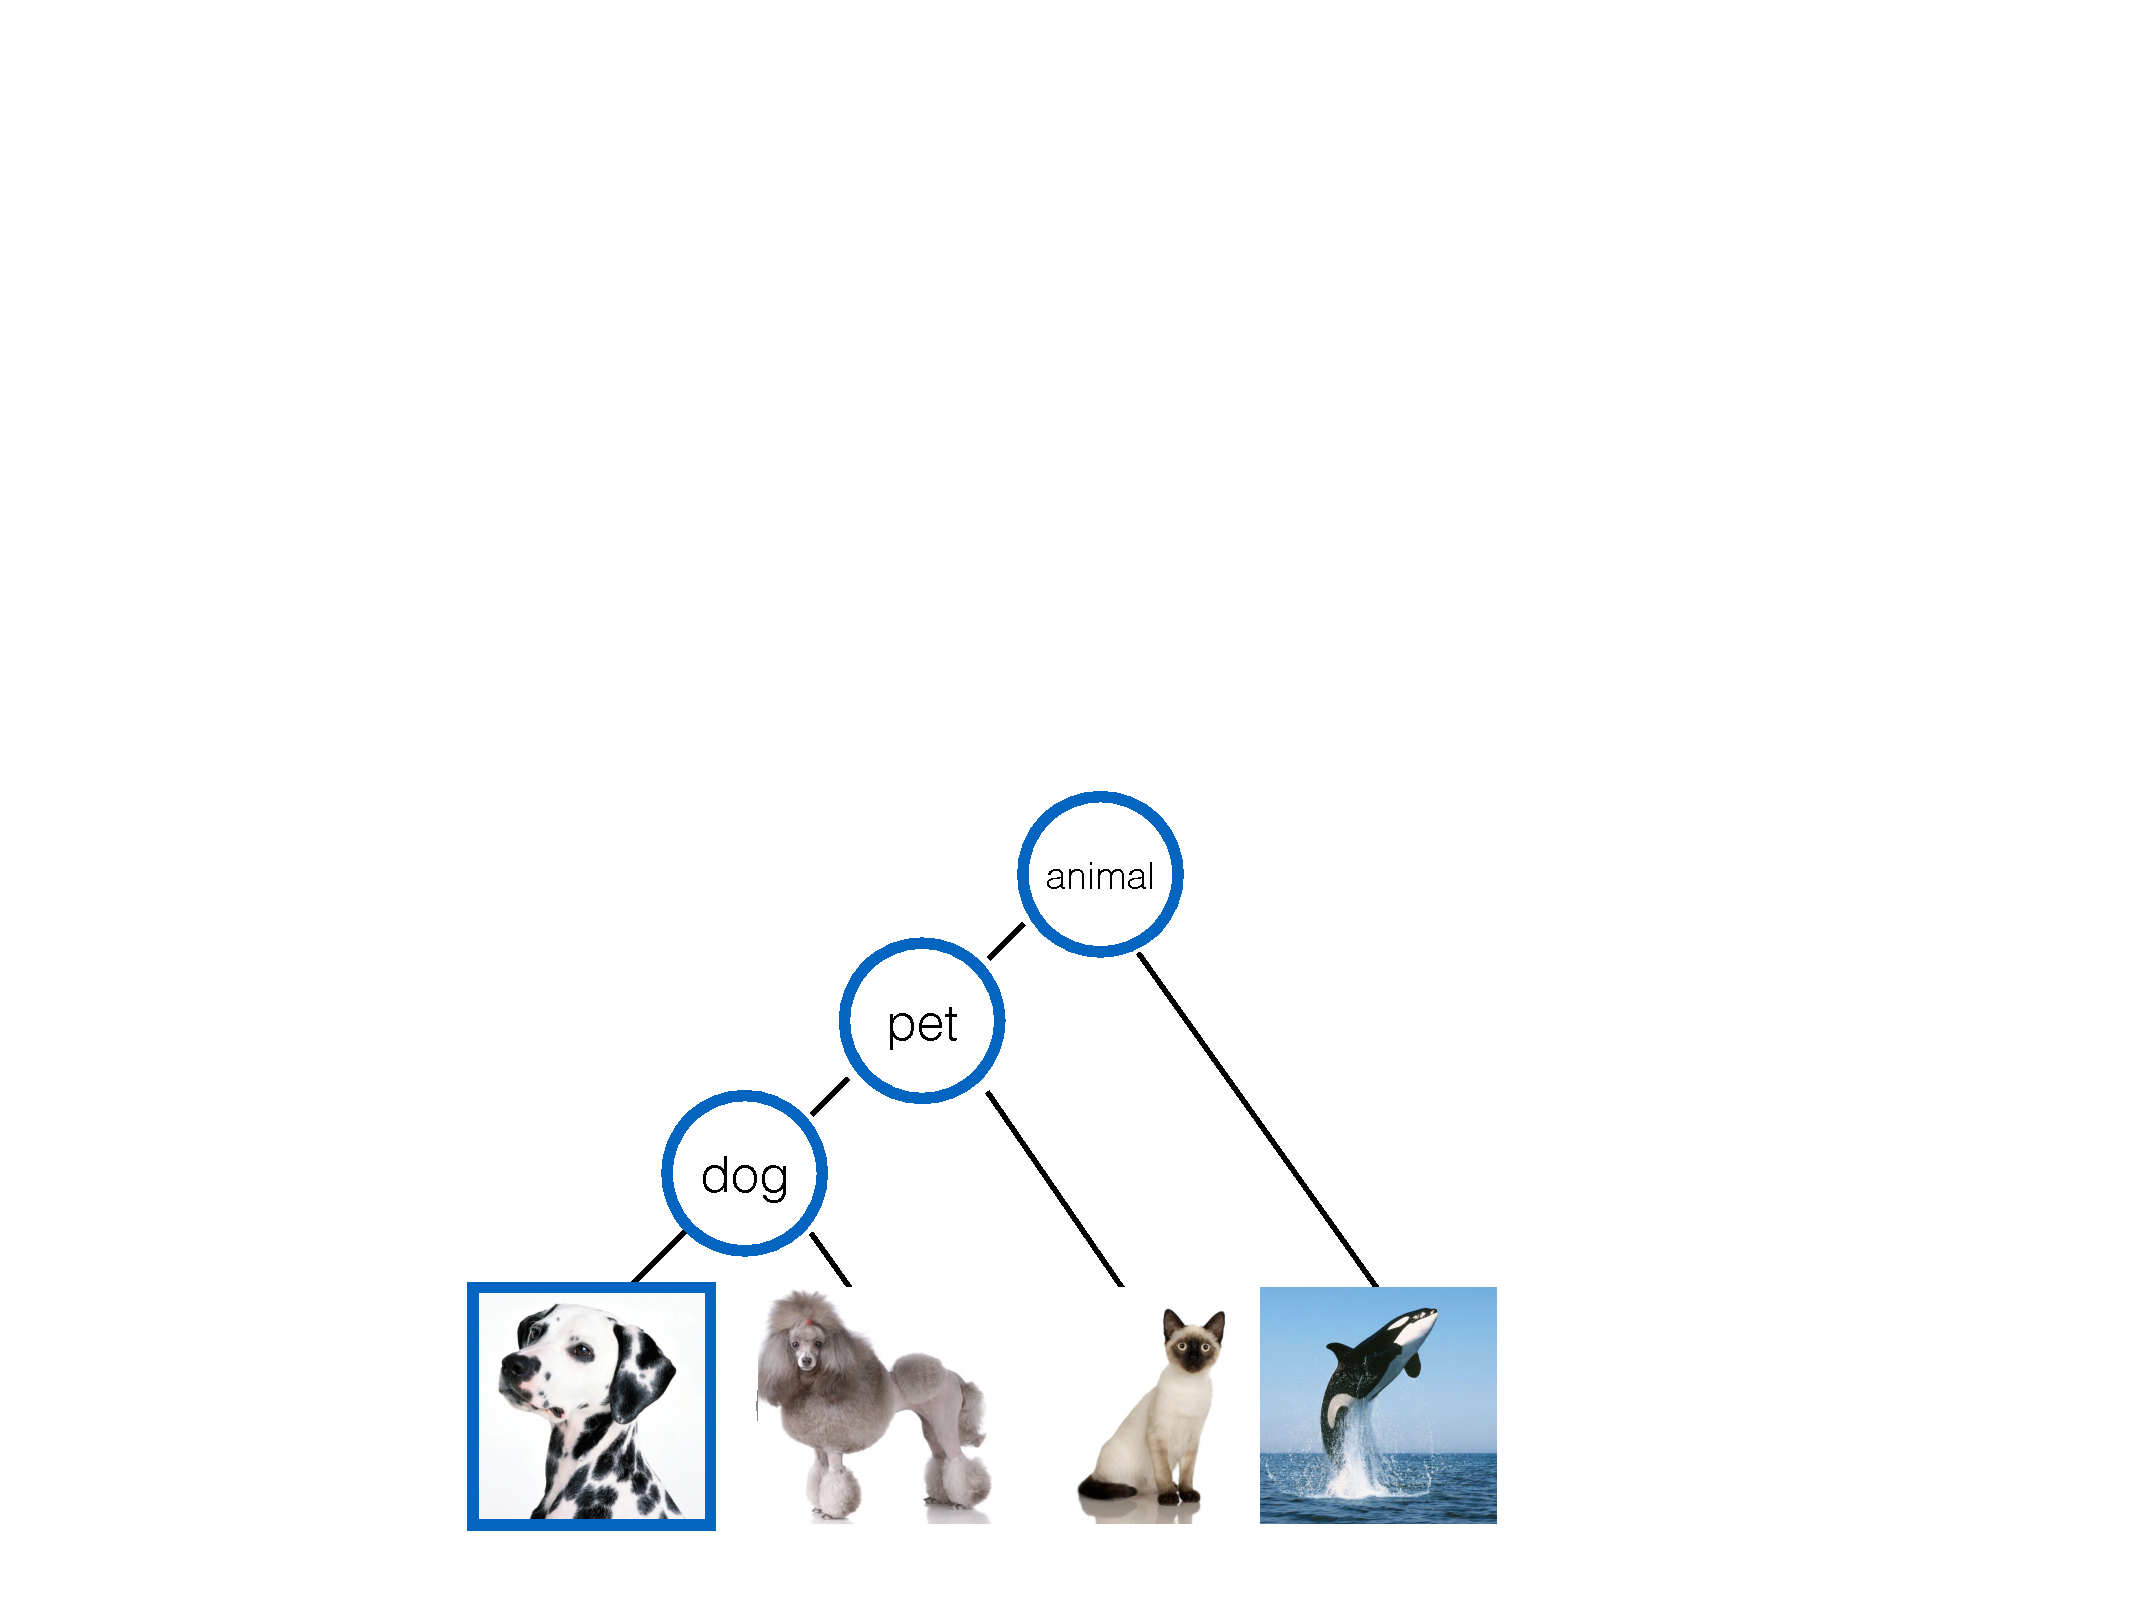
\includegraphics[scale = .35]{taskhierarchy.pdf}
\end{center}
\vspace{-.25cm}
\caption{Stimulus hierarchy used in Exp.~1. The goal space and answer space contained the four leaves. %hidden behind gates (the nodes of the tree). 
The question space, however, was restricted to the highlighted nodes, proceeding up the hierarchy, allowing for indirect questions.}
\label{fig:taskhierarchy}
\end{figure}

\subsubsection{Participants} We recruited 125 participants %between the ages of 20 and 75 
from Amazon's Mechanical Turk to participate in this task.  %They were compensated 50\textcent \, for their work, and the median completion time was 3.75 minutes. 
Eleven participants were excluded due to self-reported confusion about the task instructions or due to being non-native English speakers.

\subsubsection{Stimuli \& Procedure} In terms of our model specification, the world space $\mathcal{W}$ was the set of $4! = 24$ possible assignments of four objects to four gates. The goal space $\mathcal{G}$ was the set of four objects that the questioner could be trying to find (the leaves of the tree in Fig.~\ref{fig:taskhierarchy}). The answer space $\mathcal{A}$ was the set of four gates that the answerer could  reveal. The restricted question space $\mathcal{Q}$ contained the set of highlighted nodes in the hierarchy: `dalmatian?', `dog?', `pet?', and `animal?'. 

	\begin{figure}[t!]
\begin{center}
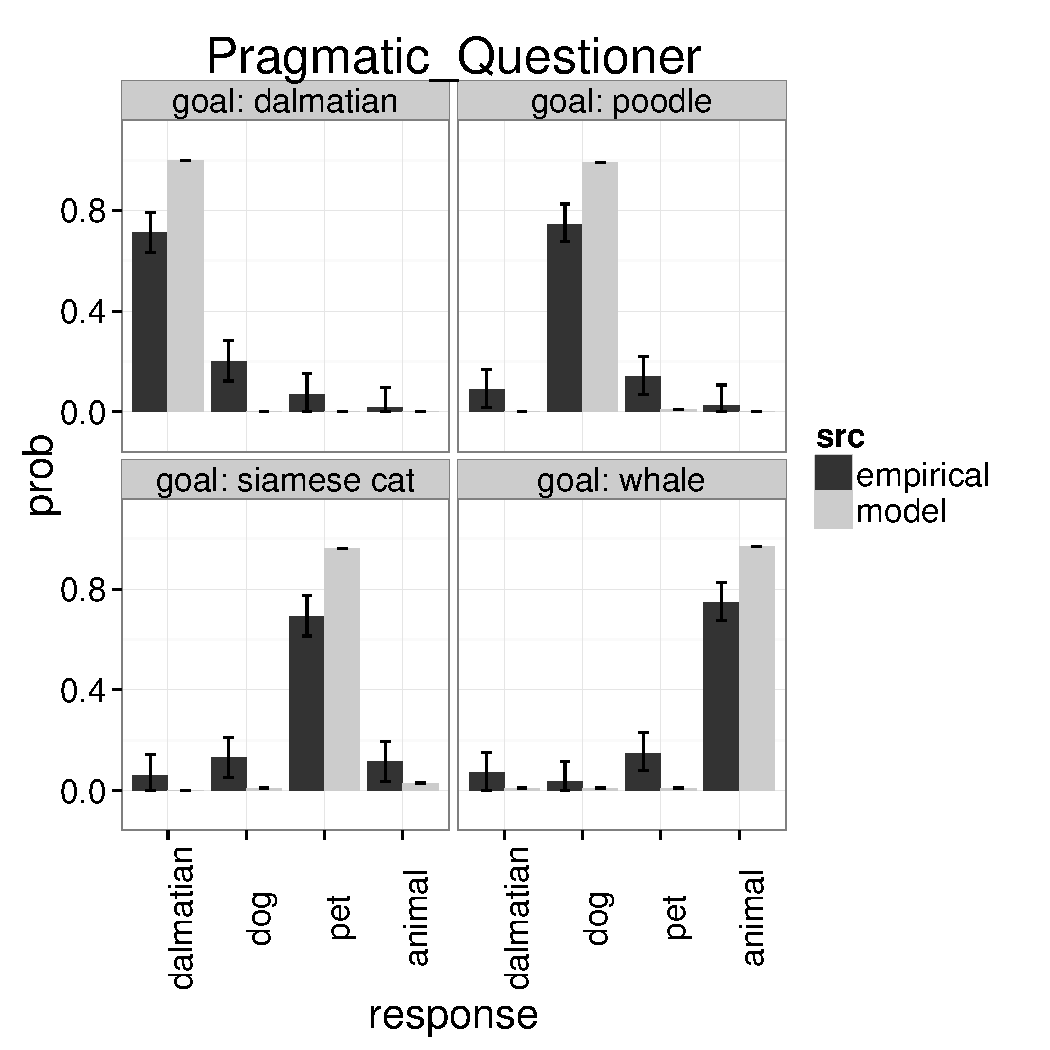
\includegraphics[scale = .4]{Exp1PragmaticQuestioner.pdf}
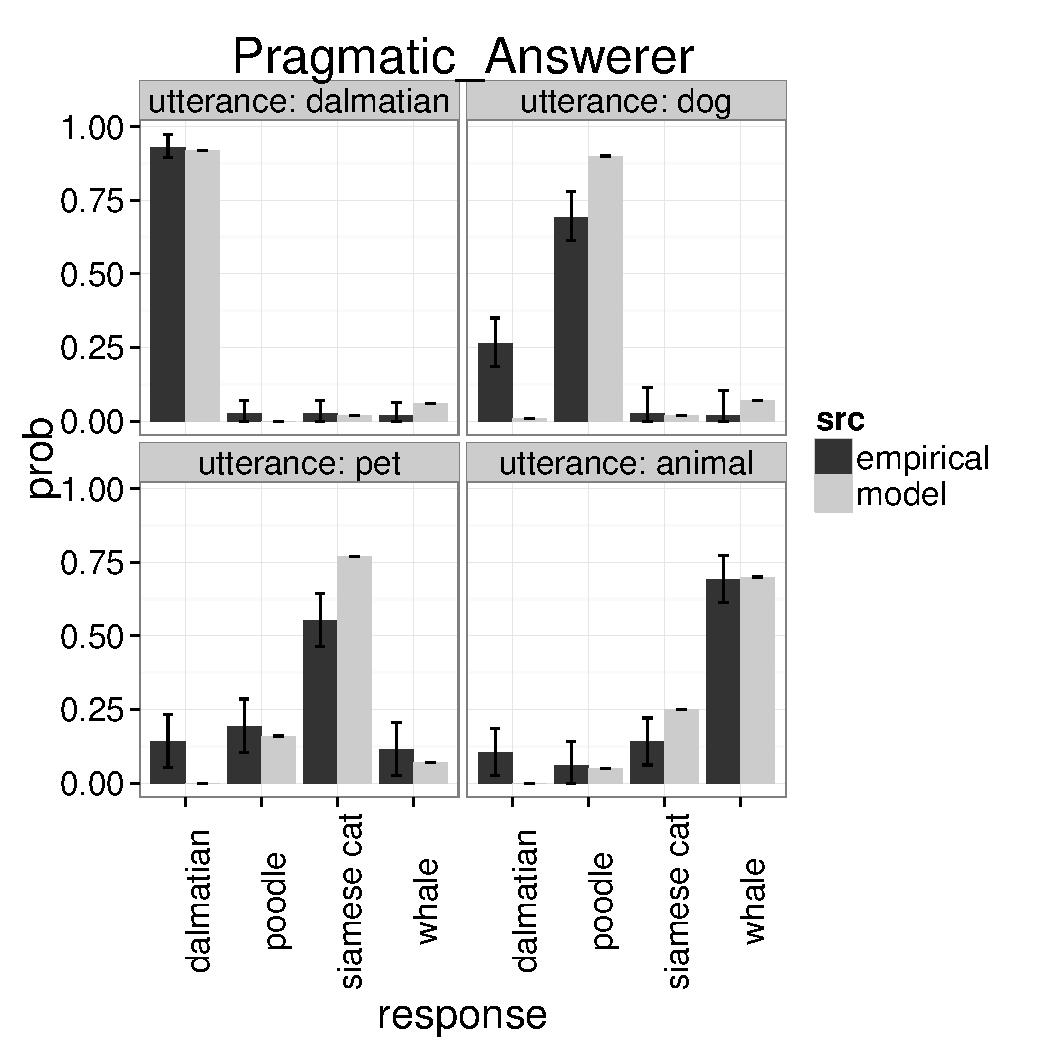
\includegraphics[scale = .4]{Exp1PragmaticAnswerer.pdf}
\end{center}
\vspace{-.5cm}
\caption{Exp.~1 results, compared with the predictions of the best-performing model  for questioner (left) and answerer (right).  The explicit and pragmatic questioner models do not make different predictions in this task, but the pragmatic answerer better accounts for the qualitative patterns in the response data than the explicit answerer.}
\vspace{-.1cm}
\label{fig:exp1res}
\end{figure}

Each participant provided responses for four trials in the role of the questioner (corresponding to the four goals), and four trials in the role of the answerer (corresponding to the four possible questions). In the questioner block, players were presented with a private goal from $\mathcal{G}$, like ``find the poodle!'' and were prompted to select a question from a drop-down menu containing elements of $\mathcal{Q}$ that would best help them find it. In the answerer block, players were shown which items were behind which gates and were told that the other player had asked a particular question from $\mathcal{Q}$. They were prompted to select a gate from a drop-down menu that would be most helpful for the questioner, keeping in mind his or her constraints. 
(To minimize learning effects, questioners did not receive answers and neither role saw the outcome of the game.%; this may have affected motivation.
)
In order to collect responses for all elements of $\mathcal{G}$ and $\mathcal{Q}$, the order of the questioner and answerer blocks was randomly assigned for each participant, and the order of stimuli within these blocks was also randomized%\footnote{The experiment is online at \url{http://cocolab.stanford.edu/cogsci2015/Q_and_A/experiment1/experiment1.html}}. 

\subsubsection{Results}
%\red{check for effect of Q/A block order.}
Results for the questioner role are shown alongside model predictions in Fig.~\ref{fig:exp1res} (left). We find that questioners systematically prefer to ask different questions given different goals, even as those questions become more indirect. $\chi^2$ tests over each of the four response distributions show a significant divergence from uniform. Questioners preferentially ask about the `dalmatian' given the  dalmatian goal, ${\chi^2(3) = 137}, {p < .001}$, about the `dog' given the poodle goal, ${\chi^2(3) = 152}, {p <.001}$, about the `pet' given the cat goal, ${\chi^2(3) = 120},  {p <.001}$, and about the `animal' when given the whale goal, ${\chi^2(3) = 150}, {p <.001}$. 

Results for the answerer role are shown in Fig.~\ref{fig:exp1res} (right). Answerers are highly sensitive to the constraints of the questioner, giving information about the dalmatian when asked about a `dalmatian', ${\chi^2(3) = 281}, {p <.001}$, about the poodle when asked about a `dog', ${\chi^2(3) = 137}, {p <.001}$, about the cat when asked about a `pet', ${\chi^2(3) = 57}, {p<.001}$, and about the whale when asked about an `animal', ${\chi^2(3) = 121}, {p < .001}$. Note that, under an explicit interpretation of the question, revealing the dalmatian and the poodle would both be perfectly acceptable answers to a question about a `dog', but answerers strongly prefer to give the location of the poodle.  In the next section, we compare these results to the predictions of our family of models (Fig. \ref{fig:Exp1ModelSpace}). 

\subsubsection{Model comparison}
Each model was run with uniform prior probability over worlds, goals, questions, and answers, and with equal cost for all utterances. For each model, a single optimality parameter, which applied to all agents as described above, was fit to maximize correlation with the data.

We can rule out both the literal answerer and literal questioner. The \emph{literal answerer} yields a uniform distribution over the four answers. %that are the case in the given world. 
This has consequences for the corresponding \emph{literal questioner} model: when this questioner reasons about which question would generate the most helpful answer from the literal answerer, it finds no differences in response probabilities, and therefore has no preference for which question to ask. The predictions of these model, plotted against our empirical results, are shown in the left-hand column of Fig. \ref{fig:Exp1ModelSpace}.
%; questioners and answerers behave very differently than predicted by these literal models, so we will not consider them further.

The two remaining questioner models make roughly the same predictions for this task, and we are not able to distinguish them on the basis of these data. 
%Since the explicit questioner is nested two levels inside the pragmatic questioner, and each agent in the pragmatic questioner's recursion could in principle be associated with a free rationality parameter, we must consider model complexity when making comparisons. 
%To ensure equal footing for the different models, we use just two rationality parameters: one shared by questioners at all levels of recursion, and one shared by answerers at all levels of recursion. 
%For each model, we tune these parameters to maximize the correlation between model and data. 
We found a model-data correlation of $r = 0.96$ for the explicit questioner and correlation of $r = 0.99$ for the pragmatic questioner. Although the pragmatic model has a slightly better fit, the two models only differ slightly in the magnitude of predictions, not in qualitatively important ways such as the rank ordering of response.
%
\begin{figure}[t!]
\begin{center}
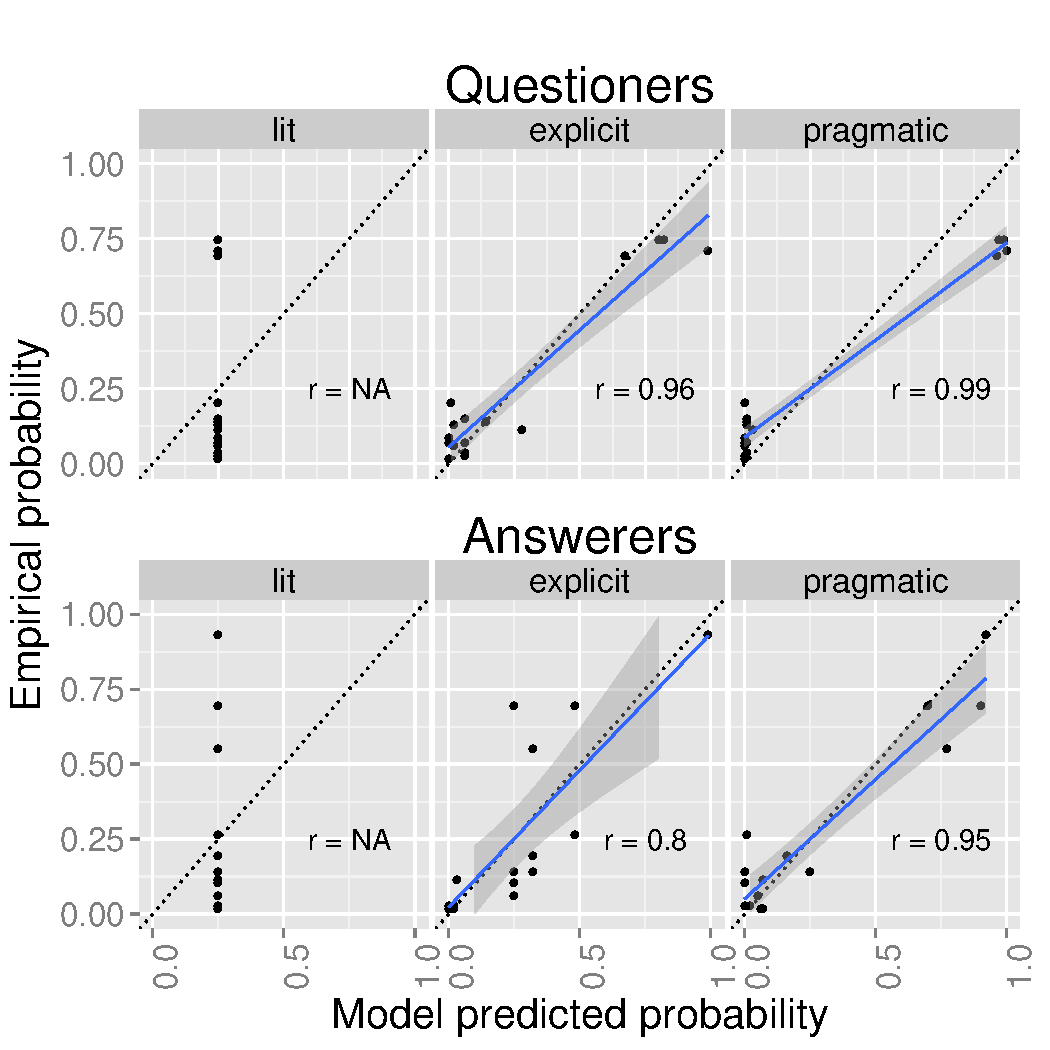
\includegraphics[scale=.75]{Exp1ModelFits.pdf}
\end{center}
\vspace{-.5cm}
\caption{Full space of models, and their correlations with the data from Exp.~1. Questioner models in the first row reason about the answerers directly below them, and the pragmatic answerer reasons about the explicit questioner.}
\label{fig:Exp1ModelSpace}
\vspace{-.15cm}
\end{figure}
%
The pragmatic questioner model's predictions for each response distribution are shown in Fig.~\ref{fig:exp1res} (left). Although the magnitude of its predictions are not in perfect alignment with the magnitude of the empirical data (because it is strongly optimizing), it captures most of the interesting qualitative patterns of the data, particularly the modal responses. 

The pragmatic answerer provides a much better fit to the data than the explicit answerer: a model-data correlation of $r = 0.8$ for the explicit answerer and $r = 0.95$ for the pragmatic answerer. 
%To ensure equal footing for model comparison, we restricted both models to a single optimality parameter, shared by all agents within the recursion.
%The model comparison here is more involved, since the explicit answerer does not depend on a questioner at all and therefore only has one parameter. We impose the same restriction on the pragmatic answerer as we applied to the pragmatic questioner, fitting one optimality parameter held in common between all answerer agents, and a second parameter for the internal questioner. 
%

\subsubsection{Discussion} Only the pragmatic answerer can account for essential qualitative features of the response data. For example, the explicit answerer predicts that participants will be equally likely to show the `dalmatian,' `poodle,' and `cat' when asked about a pet. Instead, the data show a significant preference for revealing the cat, leaving `dalmatian' and `poodle' at the same level as the other alternative. The pragmatic answerer correctly predicts this pattern  (see Fig.~\ref{fig:exp1res} (right)). Even more dramatically, the explicit answerer predicts a uniform distribution over responses to the `animal?' question. %(since all four responses denote animals)
However, the empirical distribution was significantly different from uniform. Thus, the pragmatic answerer is necessary to account for these data.

These data provide strong evidence for a pragmatic answerer, but are more equivocal with respect to the explicit and pragmatic questioner. Because the two models did not make significantly different predictions for this experiment (and both work quite well), we ran a follow-up study on a special case of the guessing-game paradigm in which the explicit and pragmatic questioners make different predictions.

\section{Exp.~2: A Critical Test of Questioner Models}

\subsubsection{Participants} We recruited 50 participants to participate only in the questioner scenario of the guessing game presented above. Ten participants were excluded on the basis of having a non-English native language, or reporting confusion about the instructions.

\subsubsection{Stimuli \& Procedure} The procedure was the same as before with some changes to the stimuli. The world space $\mathcal{W}$ consisted of possible assignments of the three pets to three gates. The possible goals $\mathcal{G}$ were the dalmatian and poodle (not the cat). The possible questions $\mathcal{G}$ were `dalmatian?' or `cat?'.  The possible answers $\mathcal{A}$ were the three gates. Each participant was given the two goals in a random order%\footnote{The experiment is online at \url{http://cocolab.stanford.edu/cogsci2015/Q_and_A/experiment2/experiment2.html}}. 

\subsubsection{Results}

When the goal was to find the dalmatian, participants were significantly more likely to ask about the dalmatian than the cat, $\chi^2(1) = 12, p < 0.001$. When the goal was to find the poodle, participants were marginally more likely to ask about the cat than the dalmatian, $\chi^2(1) = 3.6, p = 0.058$. When looking only at the first of the two trials, the dalmatian result held, $\chi^2(1) = 14.4, p < 0.001$, but participants' preference for asking about the cat disappeared, $\chi^2(1) = 0.07, p = 0.79$. These results are shown in Fig.~\ref{fig:exp2res}.

\begin{figure}[t!]
\begin{center}
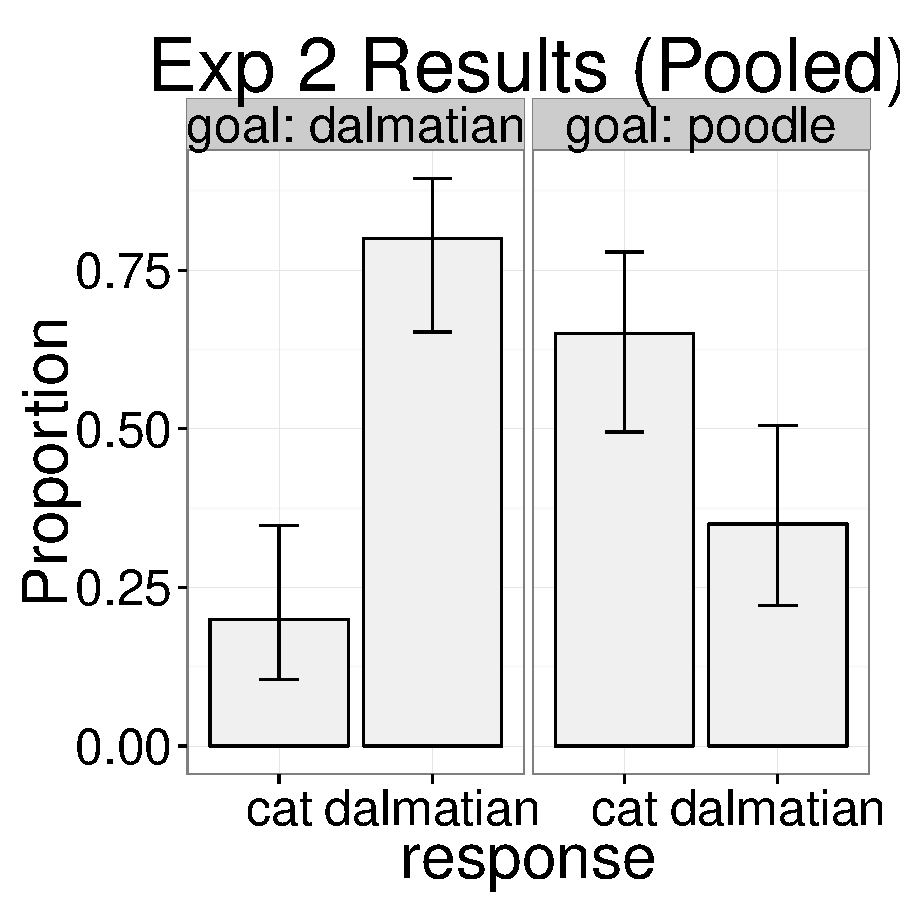
\includegraphics[scale=.45]{Exp2Results_all.pdf}
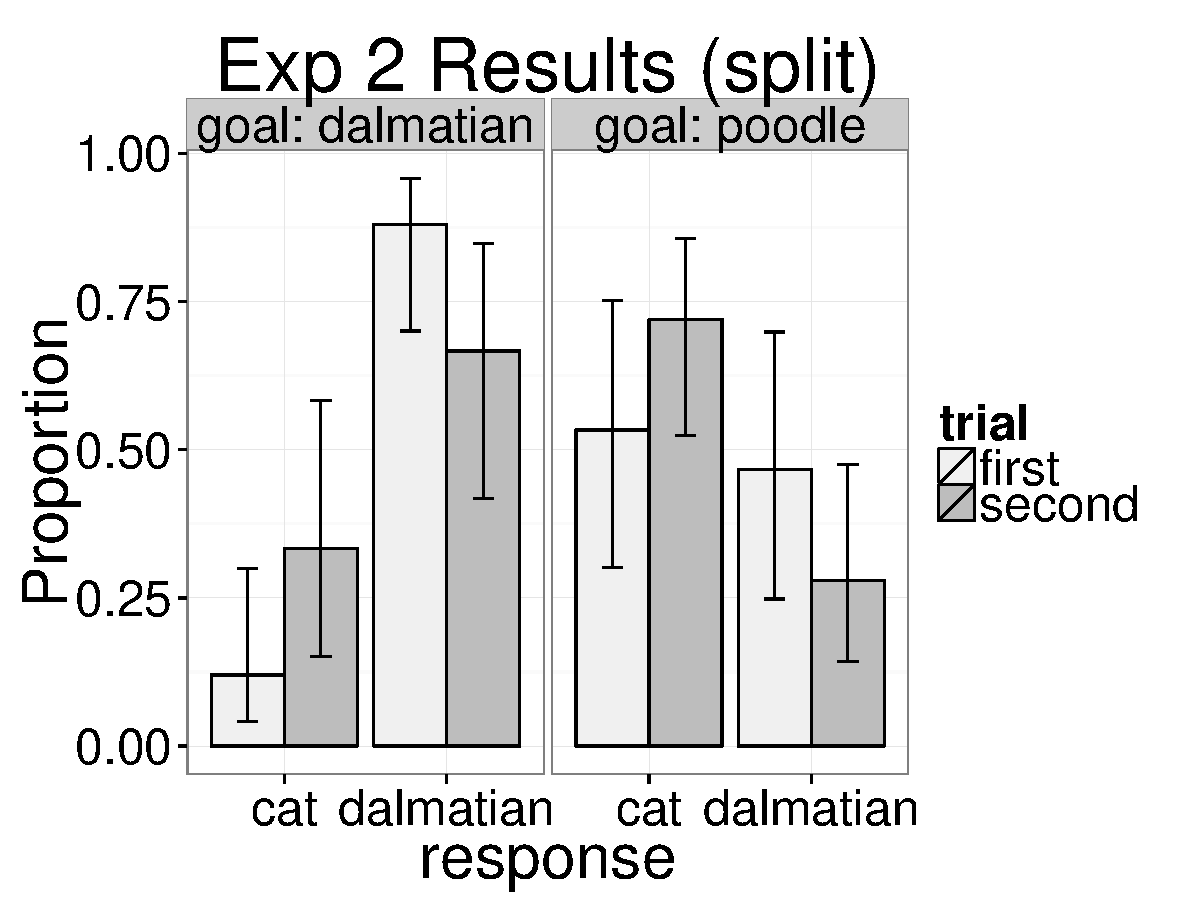
\includegraphics[scale=.45]{Exp2Results_split.pdf}
\end{center}
\vspace{-.5cm}
\caption{The overall response distribution in Exp.~2 (left) and the same distribution split into first- and second-trial data (right).}
\vspace{-.25cm}
\label{fig:exp2res}
\end{figure}

\subsubsection{Model comparison}

The explicit questioner predicts that participants should have no preference for a question given the `poodle' goal, since an explicit answerer would be equally unlikely to give the desired answer for both. The pragmatic questioner model, however, predicts that participants should prefer to ask about the cat. This is because the (internal) pragmatic answerer would reason that if the questioner was interested in the dalmatian, they would ask about the dalmatian; if they didn't, they must be interested in the other possible goal. 

It is again unclear which questioner model is best. Overall, the response distribution matches the predictions of the pragmatic model: questioners prefer to ask about the cat. 
However, participants don't show this behavior if we look at only the first trial.
This could be due to a number of reasons.
Interestingly, the pragmatic model predicts a more explicit-like response distribution if the questioner does not take into account the constraint on possible goals: if participants thought the poodle was the only goal (counter to the instructions), then asking about the dog would be consistent with the pragmatic model as well. 
It is possible that participants only fully-processed the alternative (dalmatian) goal if they had first done the trial where that was the goal.\footnote{This pattern was also replicated with a simpler set of stimuli containing red and blue squares and circles.}

\subsubsection{Discussion}

Experiment 1 established that the pragmatic answerer model is necessary to account for answerer behavior in our simple guessing-game task, complementing  results from our computational experiments. Additionally, it established that the explicit and pragmatic questioner models could capture qualitatively important features of the questioner data, such as the systematic preference for under-informative questions when the explicit label for an object was unavailable. However, both experiments 1 and 2 failed to distinguish between the explicit and pragmatic questioner models. In experiment 1, they made indistinguishable predictions; in experiment 2, the response data were confounded with participants' beliefs about goal alternatives. 

Certain aspects of the task are subject to other methodological concerns. For instance, participants only gave hypothetical judgements about what they \emph{would} say given different goals or questions instead of playing out the full game, and participants did not believe that they were playing with a real partner. These issues contributed to overall confusion about the task, and potentially reflected abstract logic-based reasoning instead of the social and linguistic intuitions we intended to test.

In the following two experiments, we modified the task in two ways to address these concerns. In experiment 3, we replicated experiment 1 in a real-time, multi-player environment where participants are assigned to either the ``questioner'' role or the ``answerer'' role and interact directly with one another as they play the full game. In experiment 4, we additionally expanded the set of items beyond the single animal hierarchy used in the previous experiments. This item set includes four different domains (animals, plants, places, and artifacts), crossed with three different hierarchy structures eliciting a larger range of predictions from our models. One of these hierarchy structures was specifically designed to provide a critical test for distinguishing the explicit and pragmatic questioner models. Unlike experiment 2, this condition did not require participants to reason about unintuitive question alternatives that do not pick out any existing items in the world. 

\section{Exp.~3: Interactive Questions and Answers}

\subsubsection{Participants} We recruited 50 participants
from Amazon's Mechanical Turk to participate in this task: 25 were assigned to the  questioner role and 25 to the answerer role, yielding 25 complete games.

\subsubsection{Stimuli \& Procedure} The world space $\mathcal{W},$ goal space $\mathcal{G}$, question space $\mathcal{Q}$, and answer space $\mathcal{A}$ were the same as in experiment 1 (see Figure \ref{fig:taskhierarchy}). The procedure was modified to accommodate real-time player-to-player interaction following \citeA{Hawkins14_RealTimeWebExperiments}. All players passed a short quiz on the game instructions and were immediately redirected to the game interface: the first player to join was assigned to be a ``questioner'' (which we called a ``guesser'' in the cover story) and told to wait until a second player was available. Once another player joined, they were assigned to be an ``answerer'' (or ``helper'') and the game began. 

	\begin{figure}[t!]
\begin{center}
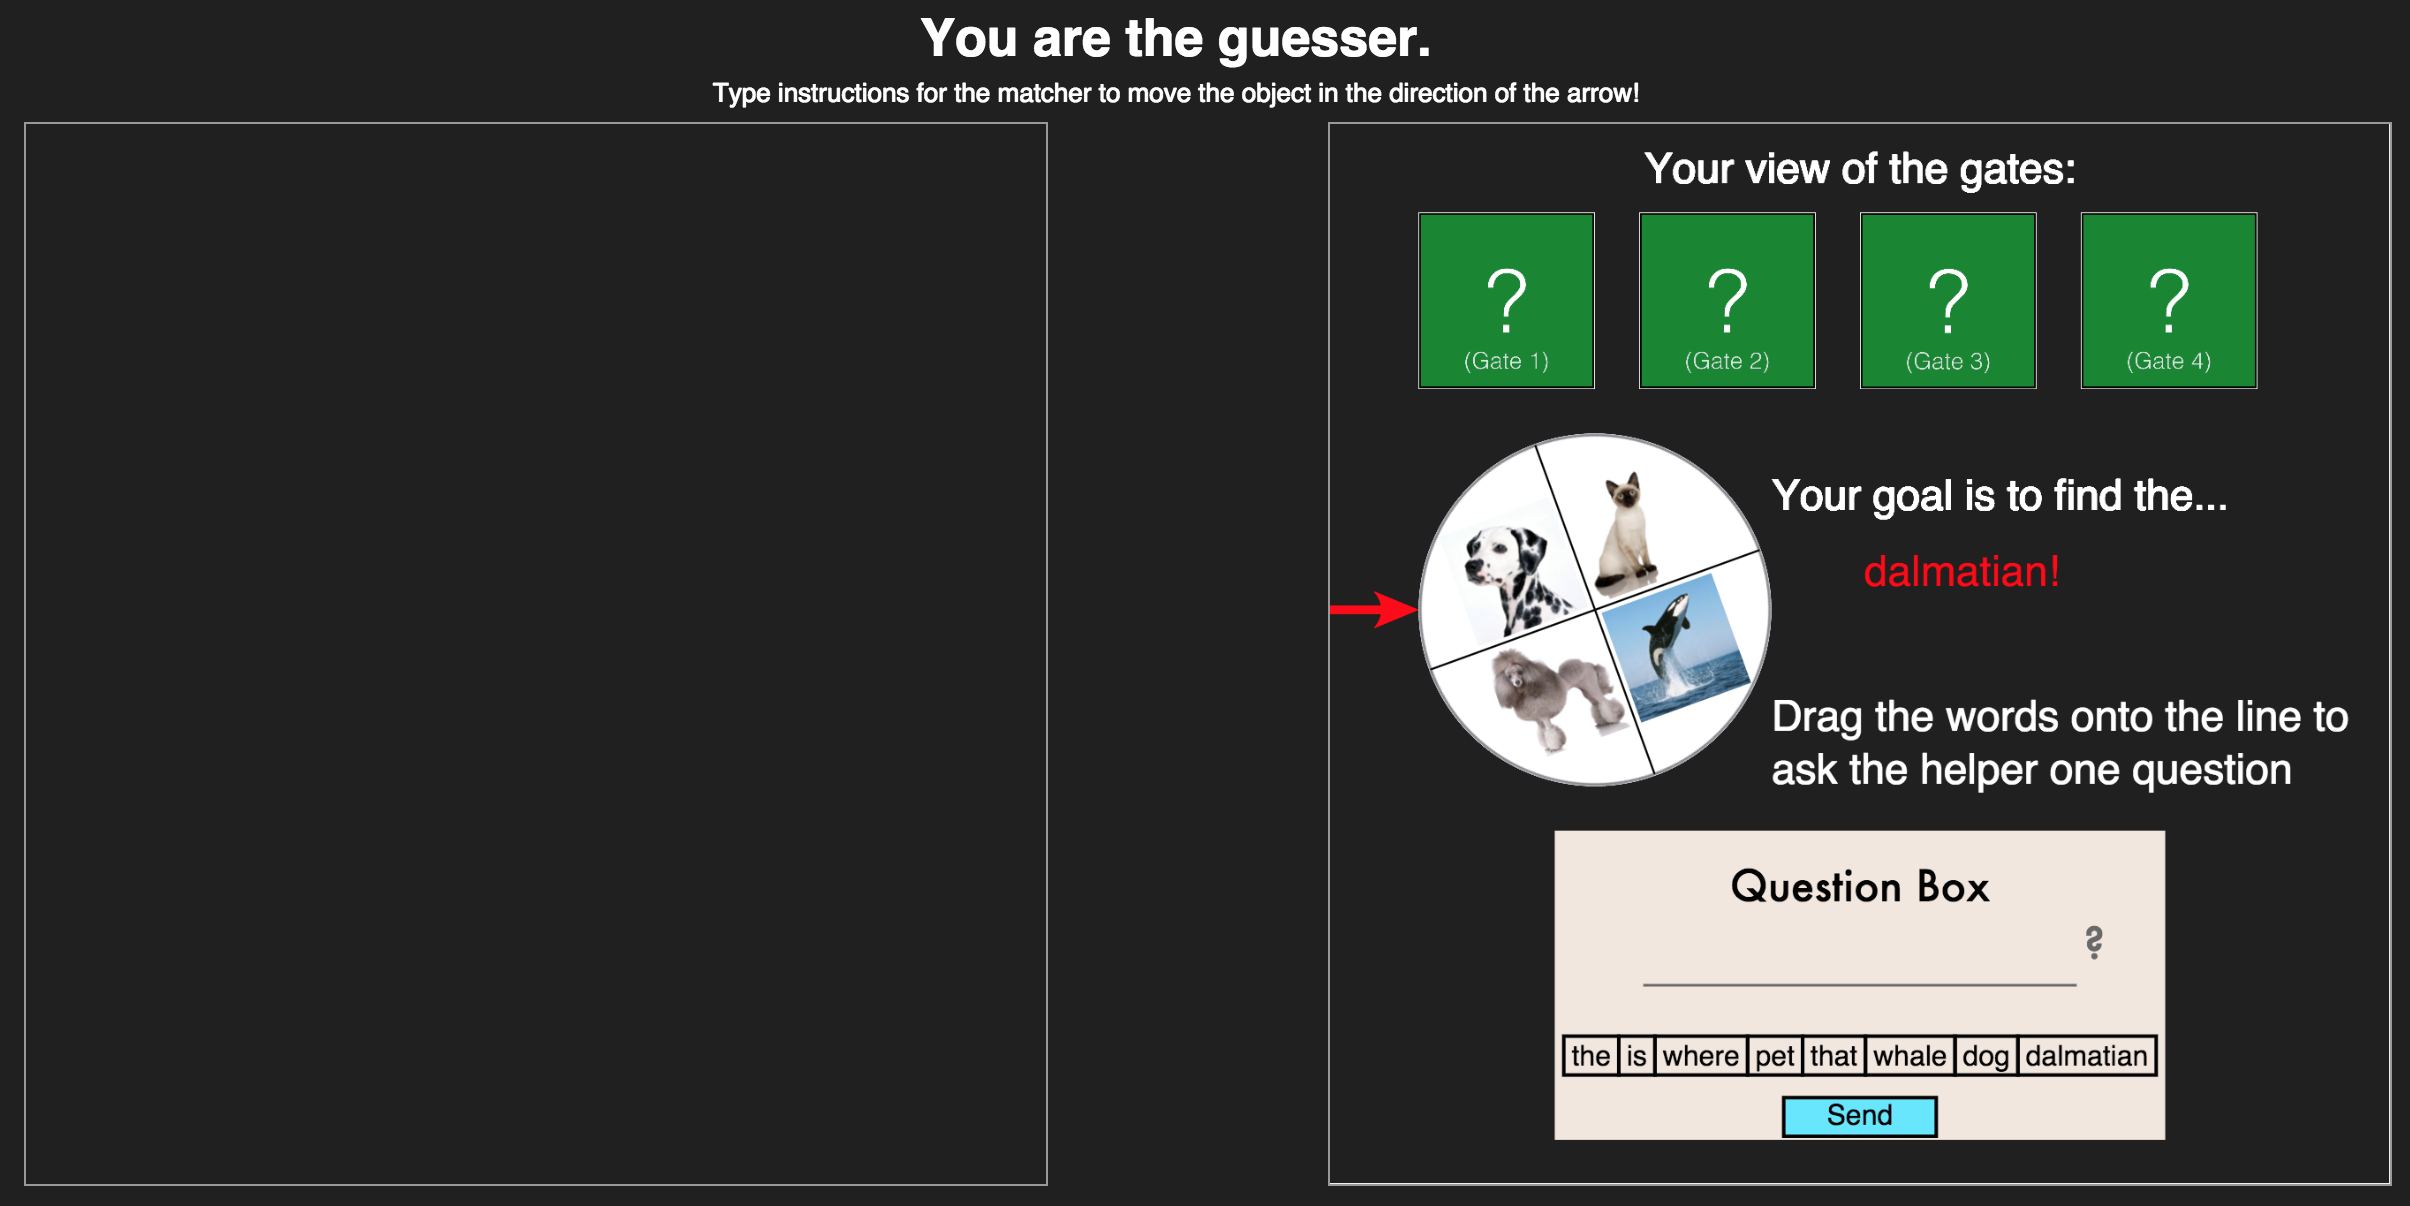
\includegraphics[scale = .3]{Exp3GuesserView}
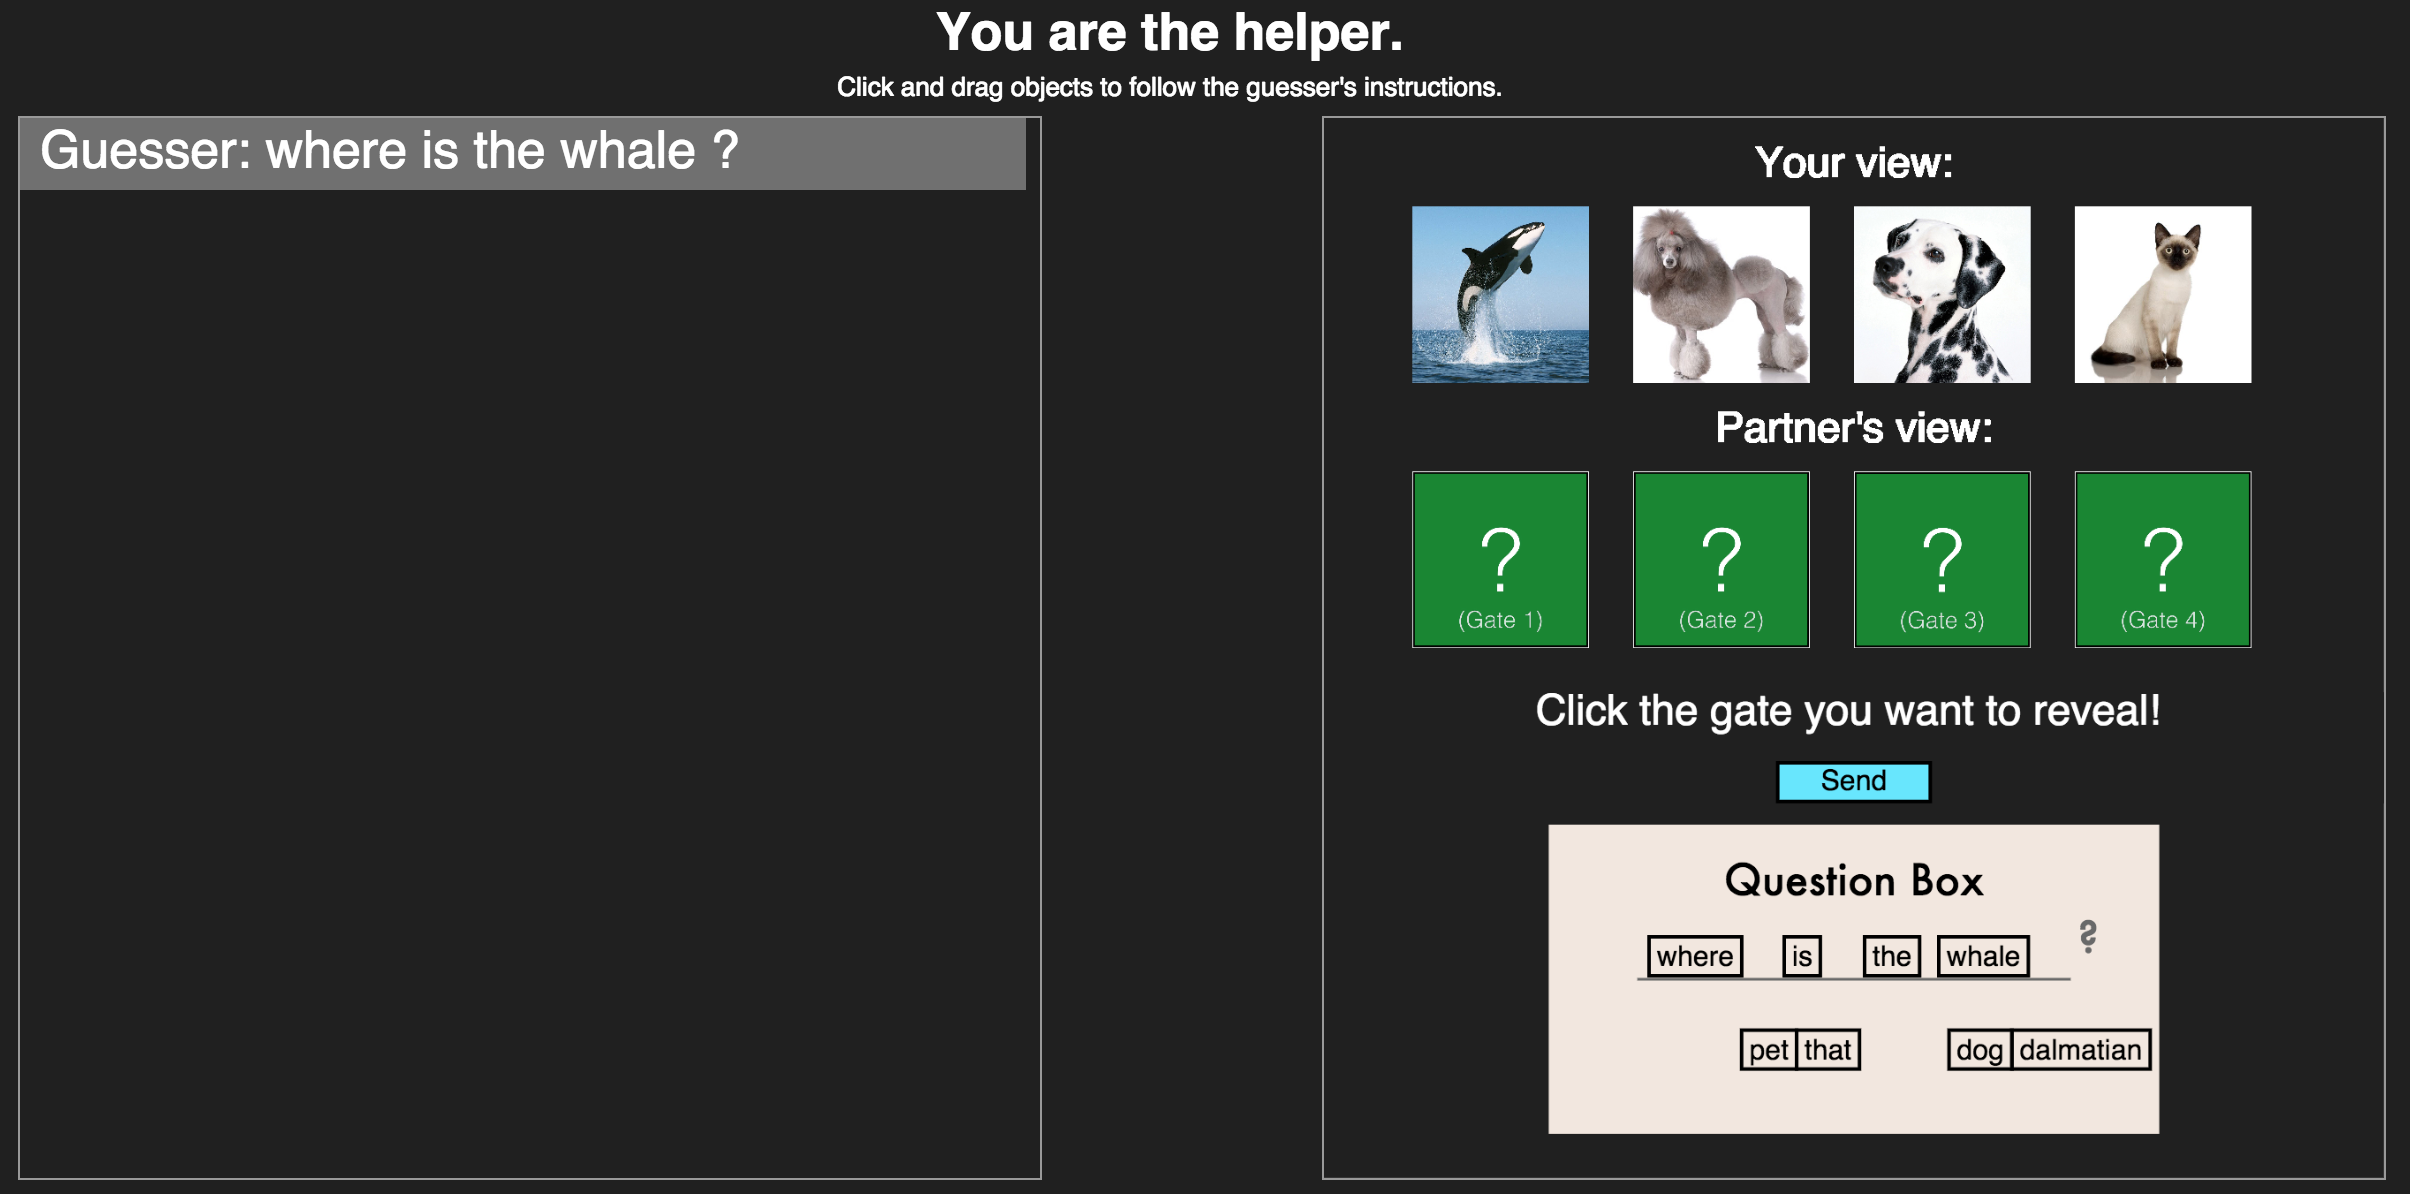
\includegraphics[scale = .3]{Exp3HelperView}
\end{center}
\vspace{-.5cm}
\caption{Exp.~3 interfaces, for the questioner (top) and answerer (bottom).}
\vspace{-.1cm}
\label{fig:exp3views}
\end{figure}

The questioner and answerer interfaces are displayed in Figure \ref{fig:exp3views}. Chat messages were printed on the left side of the screen, and players used the right side as a workspace to view goals, ask questions, and respond with answers. At the beginning of each trial, the wheel on the questioner's screen (Figure \ref{fig:exp3views}, top) would spin and select one of the four goals. The questioner then clicked and dragged words onto the line in the ``Question box'' to ask a question to help them find this goal. The answerer saw these words being dragged in real time. Once the questioner clicked the `send' button, the resulting question appeared in the chat log and control was passed to the answerer, who clicked on one of the four gates to send a response containing the location of the chosen object. Finally, the questioner was asked to guess which gate they believed the goal object was behind. 

Each participant provided responses for four trials, where object locations were shuffled and a new goal was randomly selected for each trial. Thus, questioners could be given the same goal on multiple trials, preventing `process of elimination' reasoning about what the goal may be on the part of the answerer. 

\subsubsection{Results}
%\red{check for effect of Q/A block order.}
Results for the questioner role are shown alongside model predictions in Fig.~\ref{fig:exp3res} (left). We find that questioners systematically prefer to ask different questions given different goals, even as those questions become more indirect. $\chi^2$ tests over each of the four response distributions show a significant divergence from uniform. Questioners preferentially ask about the `dalmatian' given the  dalmatian goal, ${\chi^2(3) = 77}, {p < .001}$, about the `dog' given the poodle goal, ${\chi^2(3) = 50}, {p <.001}$, about the `pet' given the cat goal, ${\chi^2(3) = 47},  {p <.001}$, and about the `animal' when given the whale goal, ${\chi^2(3) = 39}, {p <.001}$. 

Results for the answerer role are shown in Fig.~\ref{fig:exp3res} (right). Answerers are highly sensitive to the constraints of the questioner, giving information about the dalmatian when asked about a `dalmatian', ${\chi^2(3) = 102}, {p <.001}$, about the poodle when asked about a `dog', ${\chi^2(3) = 47}, {p <.001}$, about the cat when asked about a `pet', ${\chi^2(3) = 45}, {p<.001}$, and about the whale when asked about an `animal', ${\chi^2(3) = 31}, {p < .001}$. In the next section, we compare these results to the predictions of our family of models (Fig. \ref{fig:Exp3ModelSpace}). 

\begin{figure}[t!]
\begin{center}
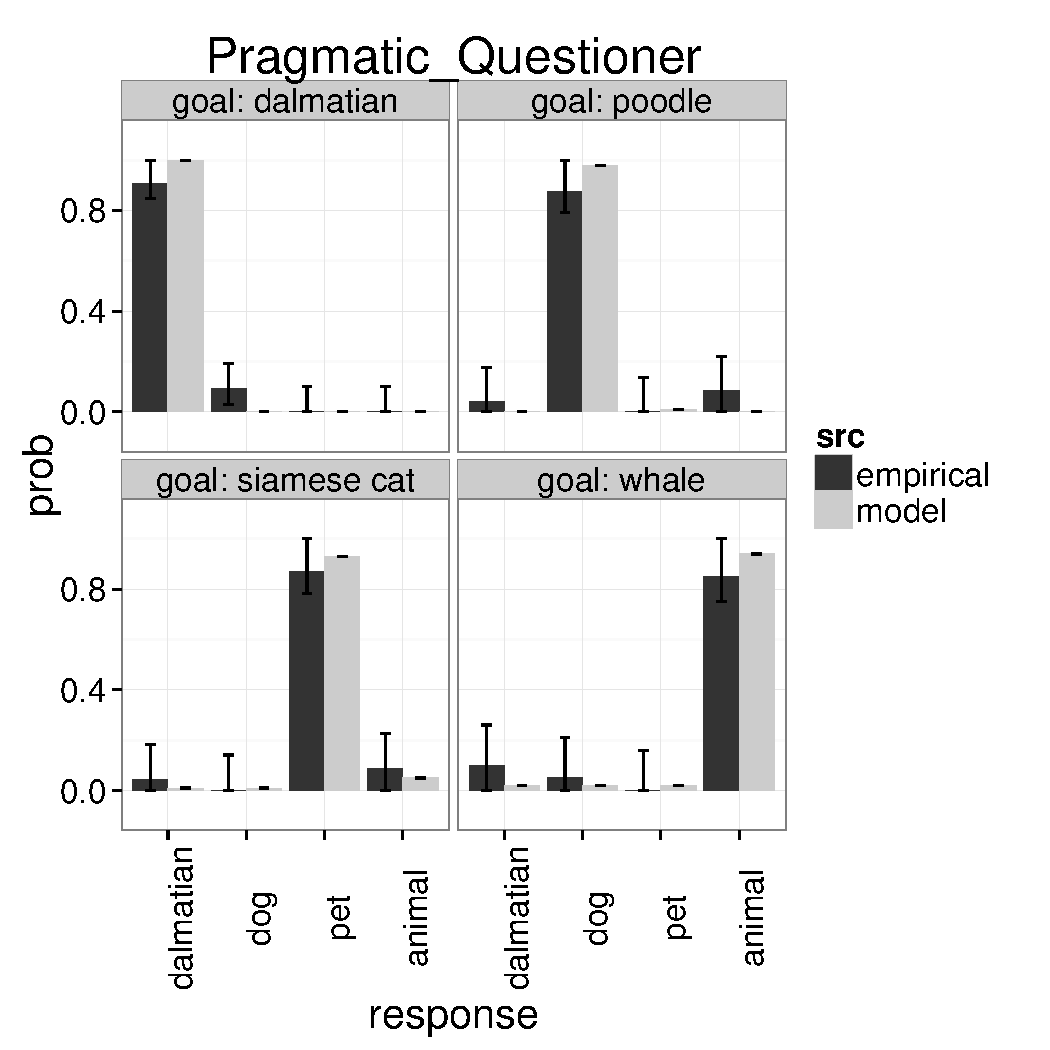
\includegraphics[scale = .4]{Exp3PragmaticQuestioner.pdf}
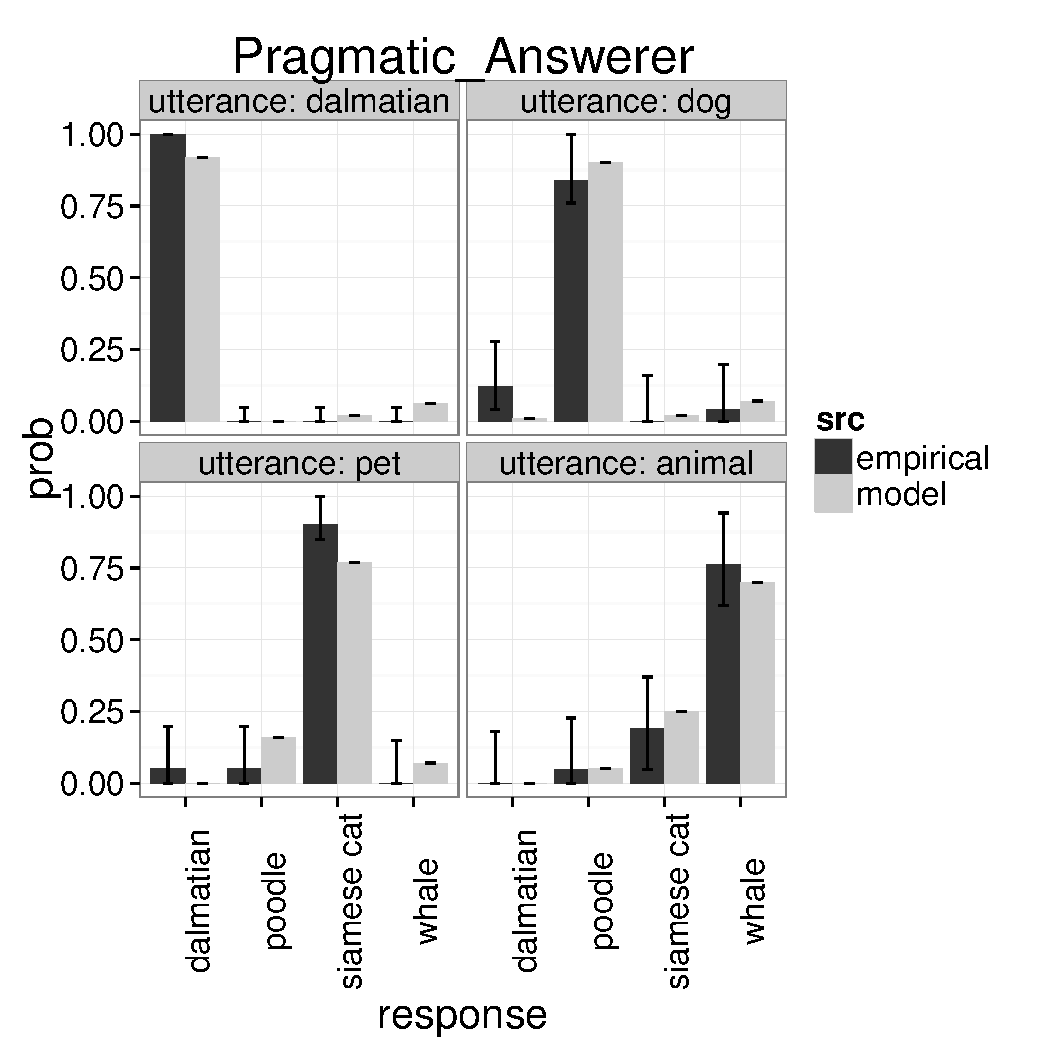
\includegraphics[scale = .4]{Exp3PragmaticAnswerer.pdf}
\end{center}
\vspace{-.5cm}
\caption{Exp.~3 results and model fits, for the best-performing questioenr (left) and answerer (right) models.}
\vspace{-.1cm}
\label{fig:exp3res}
\end{figure}

\subsubsection{Model comparison}

Model comparison was conducted in the same way as in Experiment 1: a single optimality parameter, which applied to all agents, was fit for each of the six models to maximize correlation with the data.

We can again rule out both the literal answerer and literal questioner as they predict a uniform distribution of responses over the four questions and answers. The two remaining questioner models again make roughly the same predictions for this task:
we found a model-data correlation of $r = 0.971$ for the explicit questioner and correlation of $r = 0.996$ for the pragmatic questioner. The difference between these correlations is statistically significant, accounting for their shared dependence on the empirical data (Zou's confidence interval $= [-0.079, -0.009]$). However, they make nearly identical qualitative predictions; the pragmatic questioner model's predictions for each response distribution are shown in Fig.~\ref{fig:exp3res} (left). 

The pragmatic answerer provides a much better fit to the data than the explicit answerer: we find a model-data correlation of $r = 0.7$ for the explicit answerer and $r = 0.99$ for the pragmatic answerer.  Taking into account the fact that these correlations are dependent and overlapping on the same empirical data, we find that the pragmatic answerer correlation is significantly larger than the explicit answerer correlation (Zou's confidence interval $= [-0.676, -0.107]$). 
%
\begin{figure}[t!]
\begin{center}
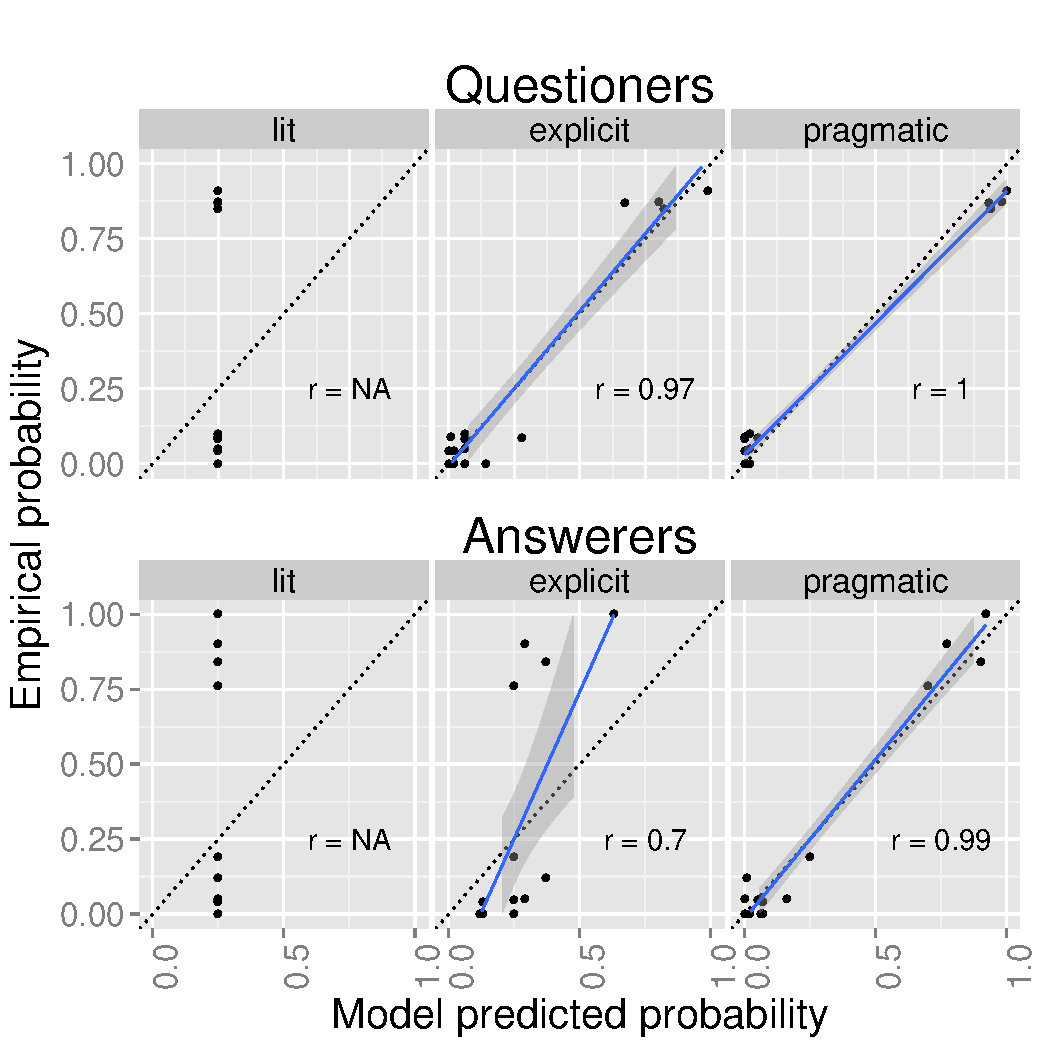
\includegraphics[scale=.75]{Exp3ModelFits.pdf}
\end{center}
\vspace{-.5cm}
\caption{Full space of models, and their correlations with the data from Exp.~1. Questioner models in the first row reason about the answerers directly below them, and the pragmatic answerer reasons about the explicit questioner.}
\label{fig:Exp3ModelSpace}
\vspace{-.15cm}
\end{figure}
%

\subsubsection{Discussion}

We replicated the results of experiment 1 in a real-time, interactive setting. Again, we found that both explicit and pragmatic questioner models provide an excellent fit to questioner behavior, and that the pragmatic answerer accounts for the data significantly better than the explicit answerer both quantitatively and qualitatively. In addition, the full, interactive game was designed to be more natural and less confusing to participants than the drop-down menu design from experiments 1 and 2. Because players received constant feedback from their partner, this task was framed as inherently social, and because answerers watched as questioners moved words to form questions, there was a convincing mechanism for people to believe they were playing with another human. This addresses some concerns raised with experiments 1 and 2. 

Note that so far we have used the same animal hierarchy for the stimulus set in all our experiments, providing only 16 points of comparison between our models and empirical data. Furthermore, there exists a heuristic strategy for selecting questions given goals in the hierarchy structure we have been using which produces the same pattern of responses without requiring any social inference. Suppose questioners saw their goal on a given trial and ruled out labels that do not apply (e.g. a `cat' is neither a `dalmatian' nor a `dog'), then picked the most specific of the remaining labels (`pet' picks out a smaller set of objects than `animal').  
 
In experiment 4, we test the generality of our model by expanding the stimulus set to encompass multiple stimulus domains and multiple hierarchy structures. This addresses the potential concern that the behavioral patterns we have been modeling are specific to the set of animals we decided to use or the tree-like hierarchy in which they were embedded. We also took care to include one simple but critical hierarchy structure where (1) the explicit and pragmatic questioner models make different predictions and (2) the heuristic strategy cannot explain these predictions. 

\section{Exp.~4: Generalizing Predictions}

\subsubsection{Participants} We recruited 191 participants
from Amazon's Mechanical Turk to participate in this task. Forty-two participants were excluded due to a server crash that terminated the task before completion. Two additional participants were excluded because they were not non-native English speakers.

\subsubsection{Stimuli \& Procedure} A set of twelve items were created by crossing four domains (animals, plants, places, and artifacts) with three hierarchy structures (``branching'', ``overlapping'', and ``equivocal''; see Figure \ref{hierarchyStructures}). For each item, there was a set of four goal objects in $\mathcal{G}$, which appeared on the wheel for the questioners, four question labels in $\mathcal{Q}$ that the questioner could use to ask about their assigned goal, and four answers in $\mathcal{A}$ corresponding to the four items in $\mathcal{G}$ that appear on the wheel.\footnote{A document containing these mappings for all items, as well as their hierarchical relationships, is available online at \url{https://github.com/hawkrobe/Q\_and\_A/blob/master/MultiExperiment2/stimuliLabels.pdf}}


 The procedure was modified to accommodate real-time player-to-player interaction following \citeA{Hawkins14_RealTimeWebExperiments}. All players passed a short quiz on the game instructions and were immediately redirected to the game interface: the first player to join was assigned to be a ``questioner'' (which we called a ``guesser'' in the cover story) and told to wait until a second player was available. Once another player joined, they were assigned to be an ``answerer'' (or ``helper'') and the game began. 

	\begin{figure}[t!]
\begin{center}
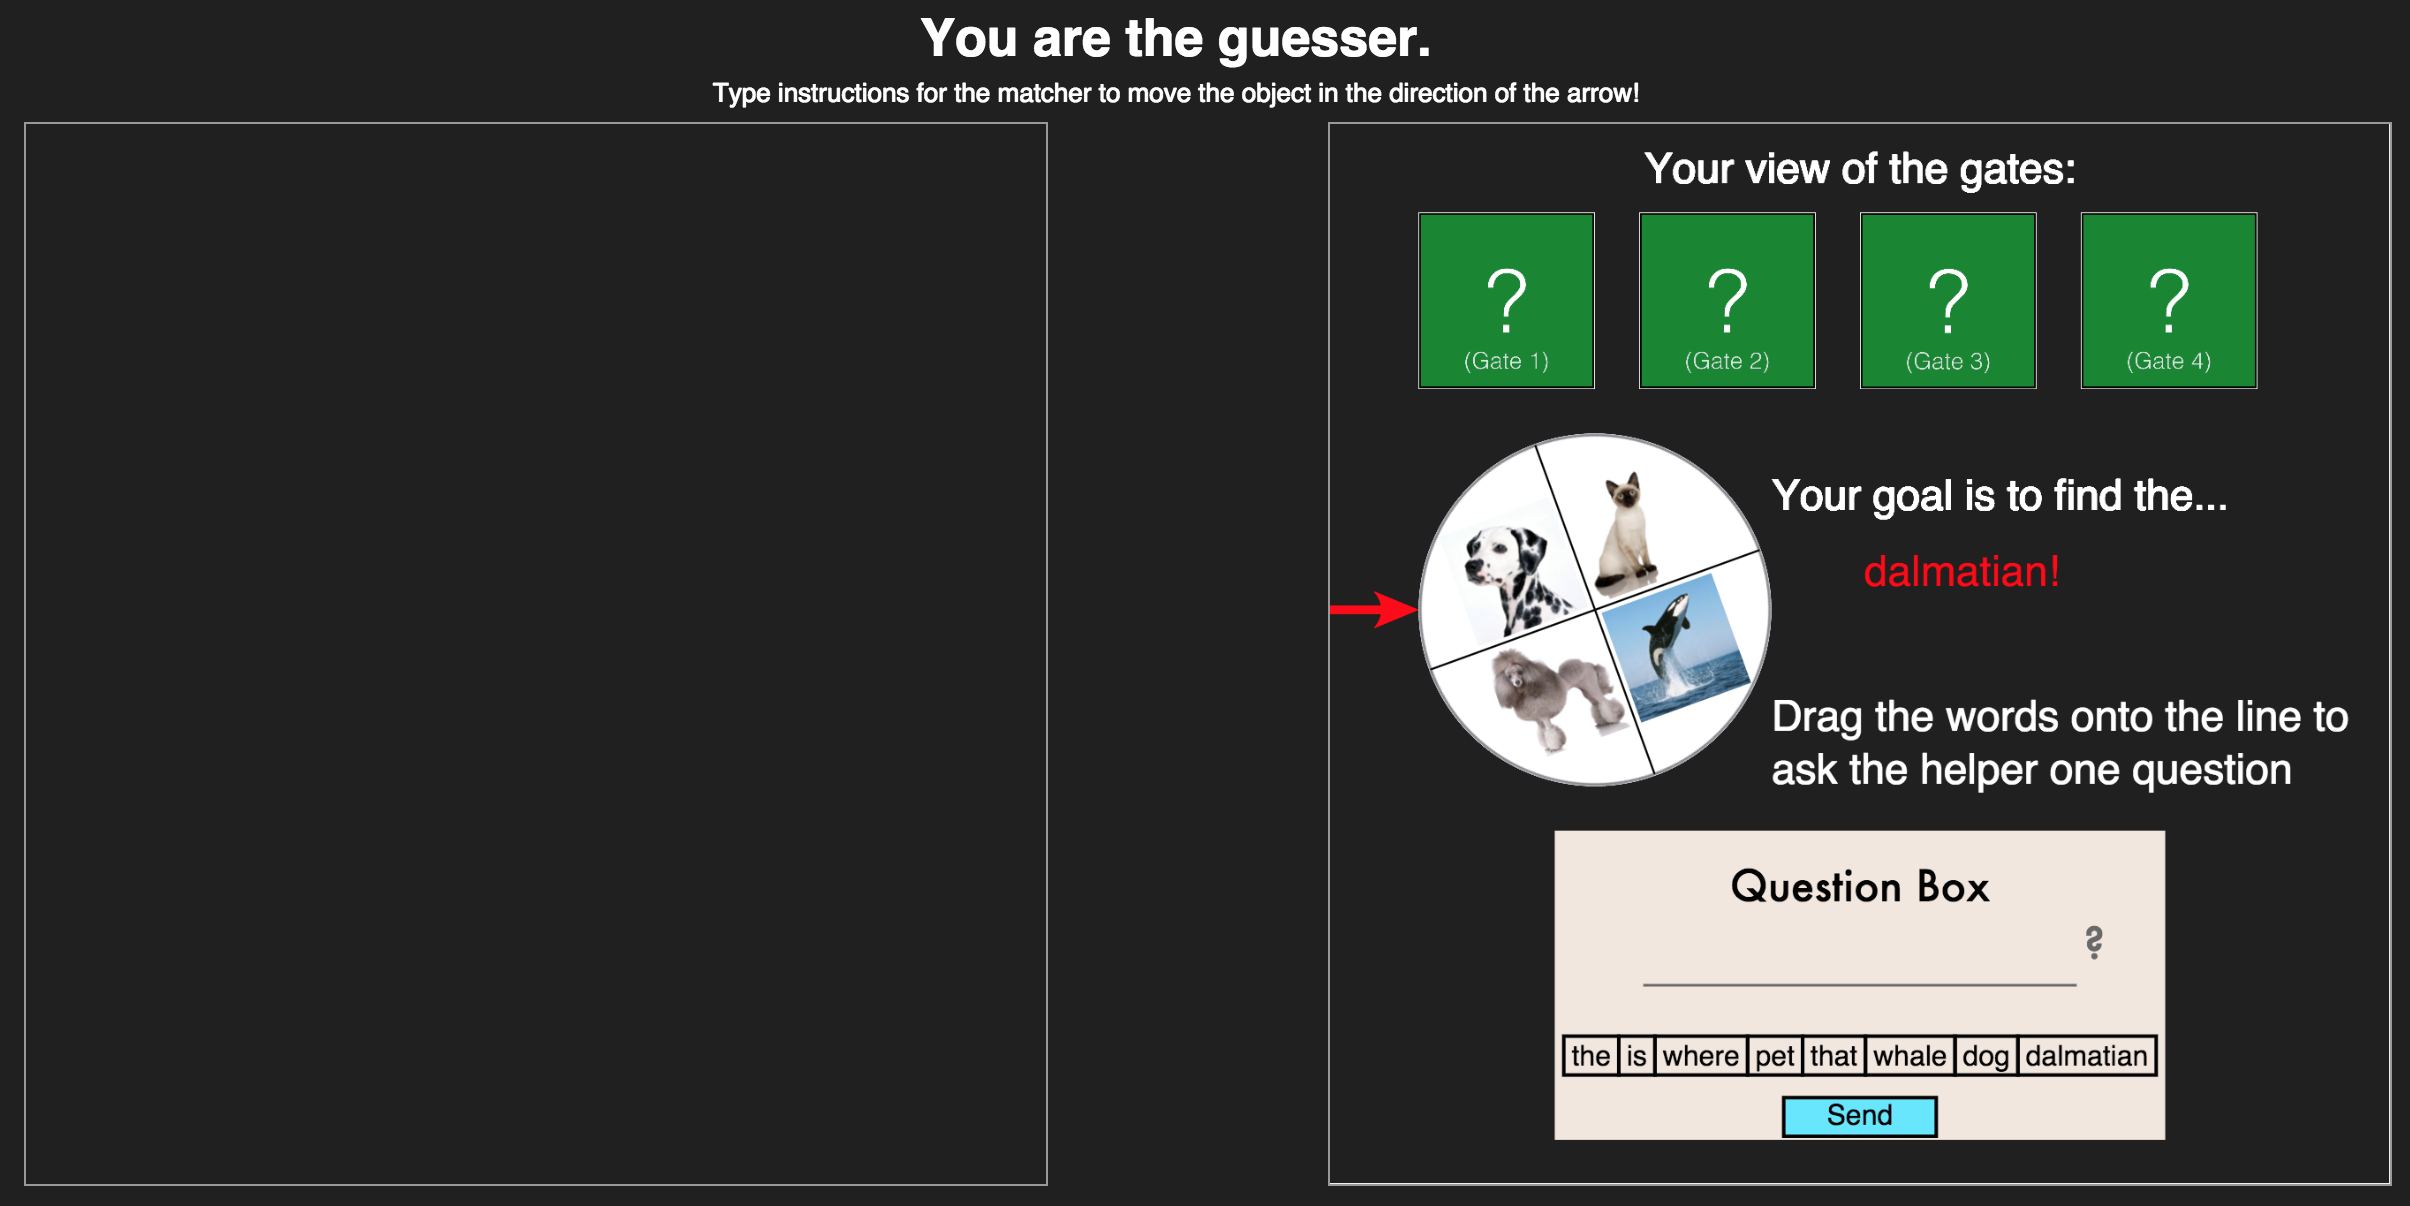
\includegraphics[scale = .3]{Exp3GuesserView}
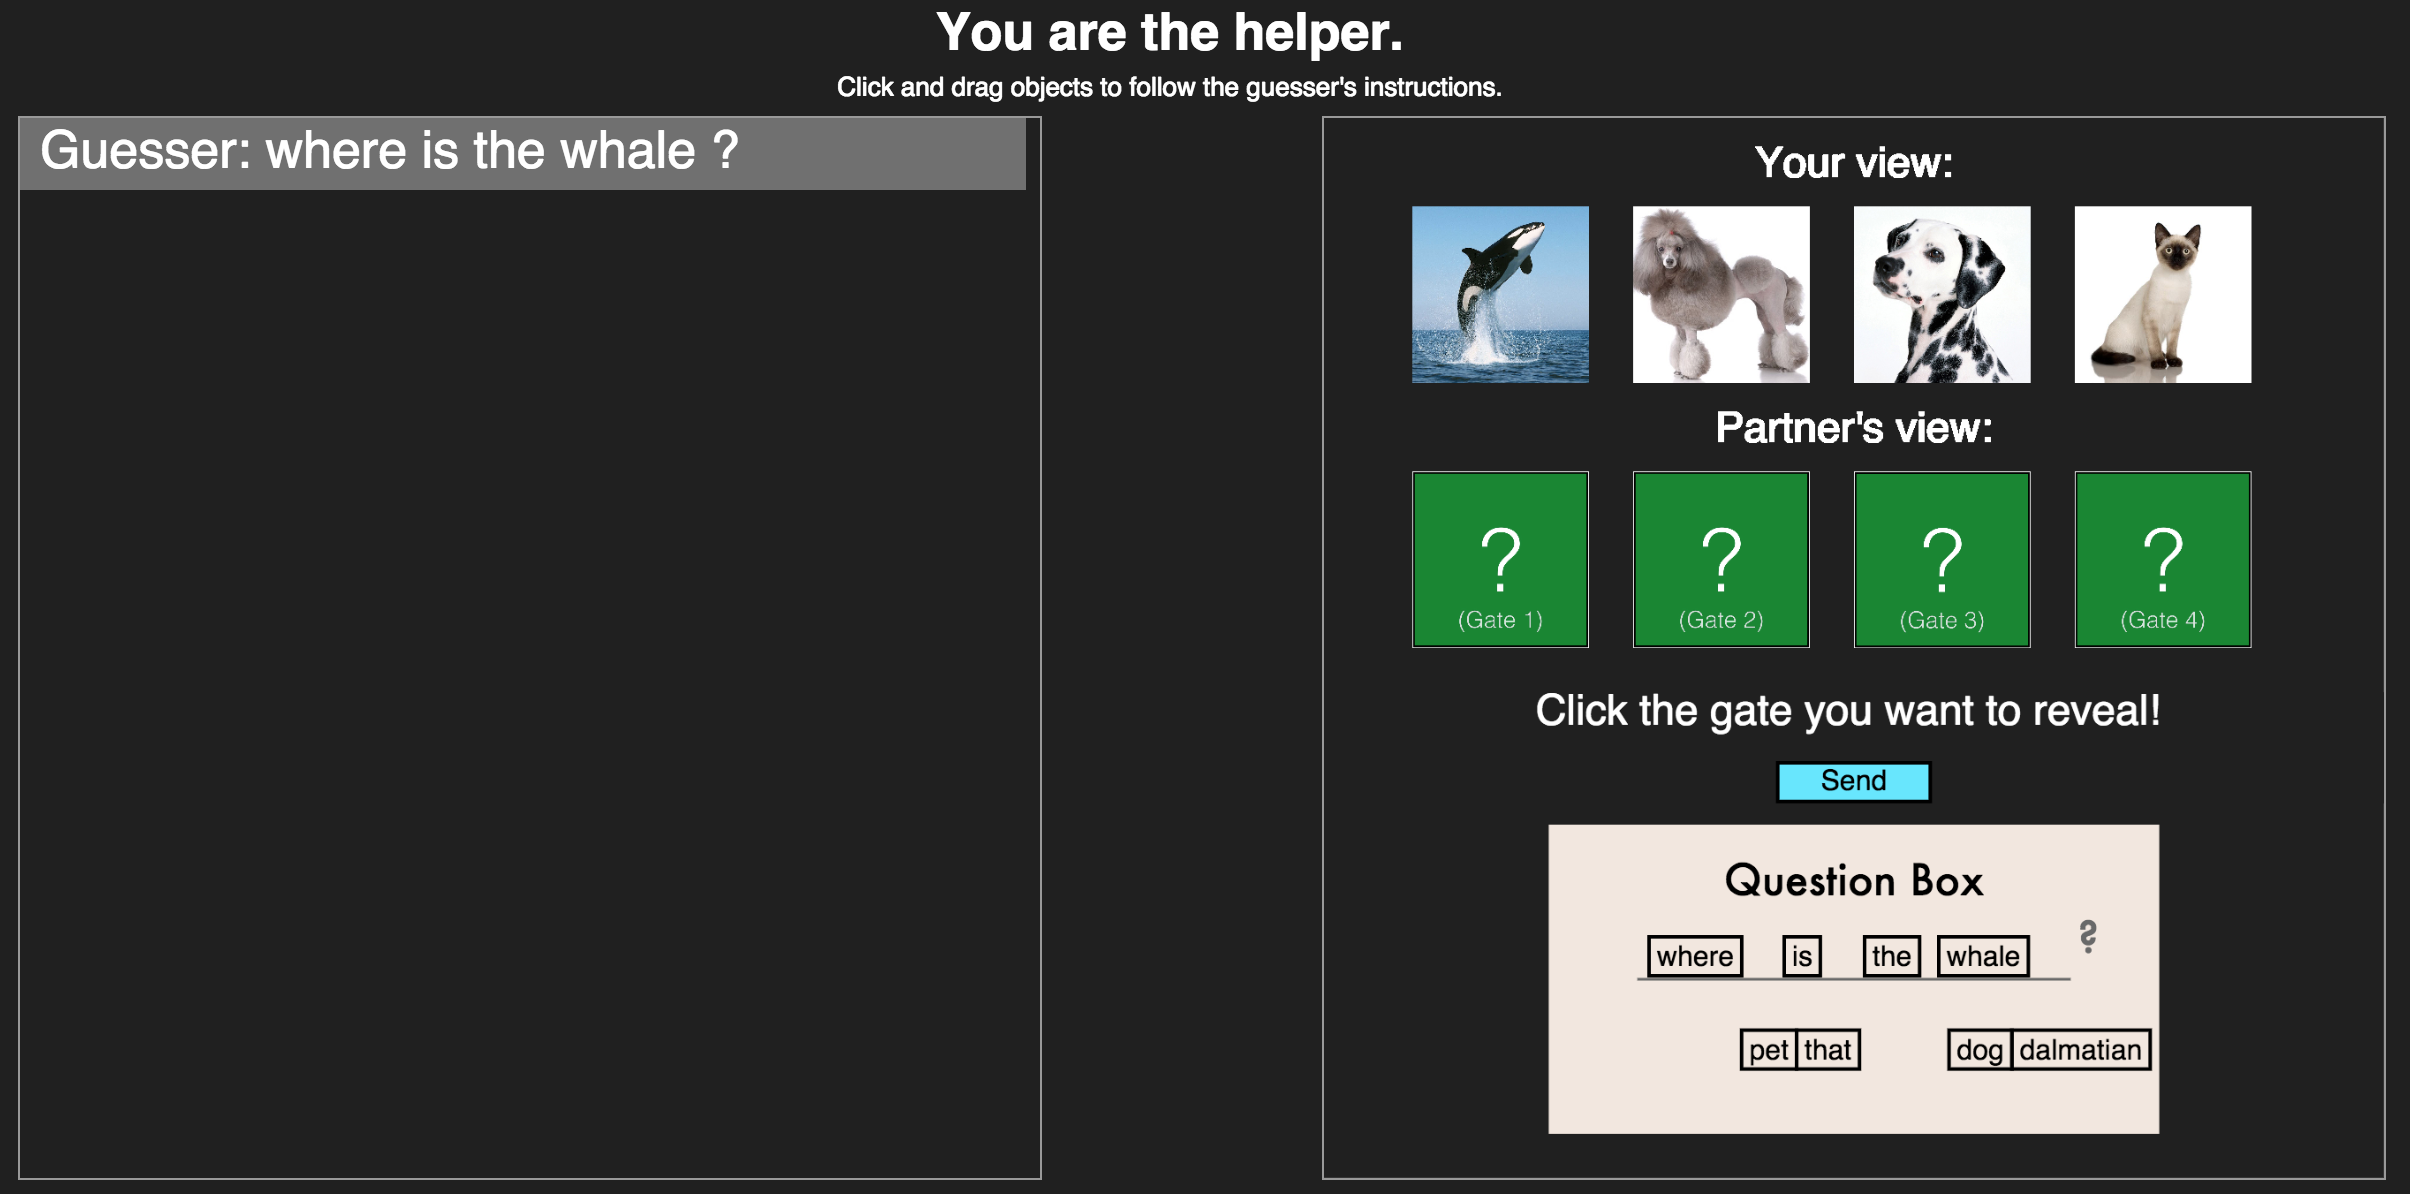
\includegraphics[scale = .3]{Exp3HelperView}
\end{center}
\vspace{-.5cm}
\caption{Exp.~3 interfaces, for the questioner (top) and answerer (bottom).}
\vspace{-.1cm}
\label{fig:exp3views}
\end{figure}

The questioner and answerer interfaces are displayed in Figure \ref{fig:exp3views}. Chat messages were printed on the left side of the screen, and players used the right side as a workspace to view goals, ask questions, and respond with answers. At the beginning of each trial, the wheel on the questioner's screen (Figure \ref{fig:exp3views}, top) would spin and select one of the four goals. The questioner then clicked and dragged words onto the line in the ``Question box'' to ask a question to help them find this goal. The answerer saw these words being dragged in real time. Once the questioner clicked the `send' button, the resulting question appeared in the chat log and control was passed to the answerer, who clicked on one of the four gates to send a response containing the location of the chosen object. Finally, the questioner was asked to guess which gate they believed the goal object was behind. 

Each participant provided responses for four trials, where object locations were shuffled and a new goal was randomly selected for each trial. Thus, questioners could be given the same goal on multiple trials, preventing `process of elimination' reasoning about what the goal may be on the part of the answerer. 

\subsubsection{Results}
%\red{check for effect of Q/A block order.}
Results for the questioner role are shown alongside model predictions in Fig.~\ref{fig:exp3res} (left). We find that questioners systematically prefer to ask different questions given different goals, even as those questions become more indirect. $\chi^2$ tests over each of the four response distributions show a significant divergence from uniform. Questioners preferentially ask about the `dalmatian' given the  dalmatian goal, ${\chi^2(3) = 77}, {p < .001}$, about the `dog' given the poodle goal, ${\chi^2(3) = 50}, {p <.001}$, about the `pet' given the cat goal, ${\chi^2(3) = 47},  {p <.001}$, and about the `animal' when given the whale goal, ${\chi^2(3) = 39}, {p <.001}$. 

Results for the answerer role are shown in Fig.~\ref{fig:exp3res} (right). Answerers are highly sensitive to the constraints of the questioner, giving information about the dalmatian when asked about a `dalmatian', ${\chi^2(3) = 102}, {p <.001}$, about the poodle when asked about a `dog', ${\chi^2(3) = 47}, {p <.001}$, about the cat when asked about a `pet', ${\chi^2(3) = 45}, {p<.001}$, and about the whale when asked about an `animal', ${\chi^2(3) = 31}, {p < .001}$. In the next section, we compare these results to the predictions of our family of models (Fig. \ref{fig:Exp3ModelSpace}). 

\begin{figure}[t!]
\begin{center}
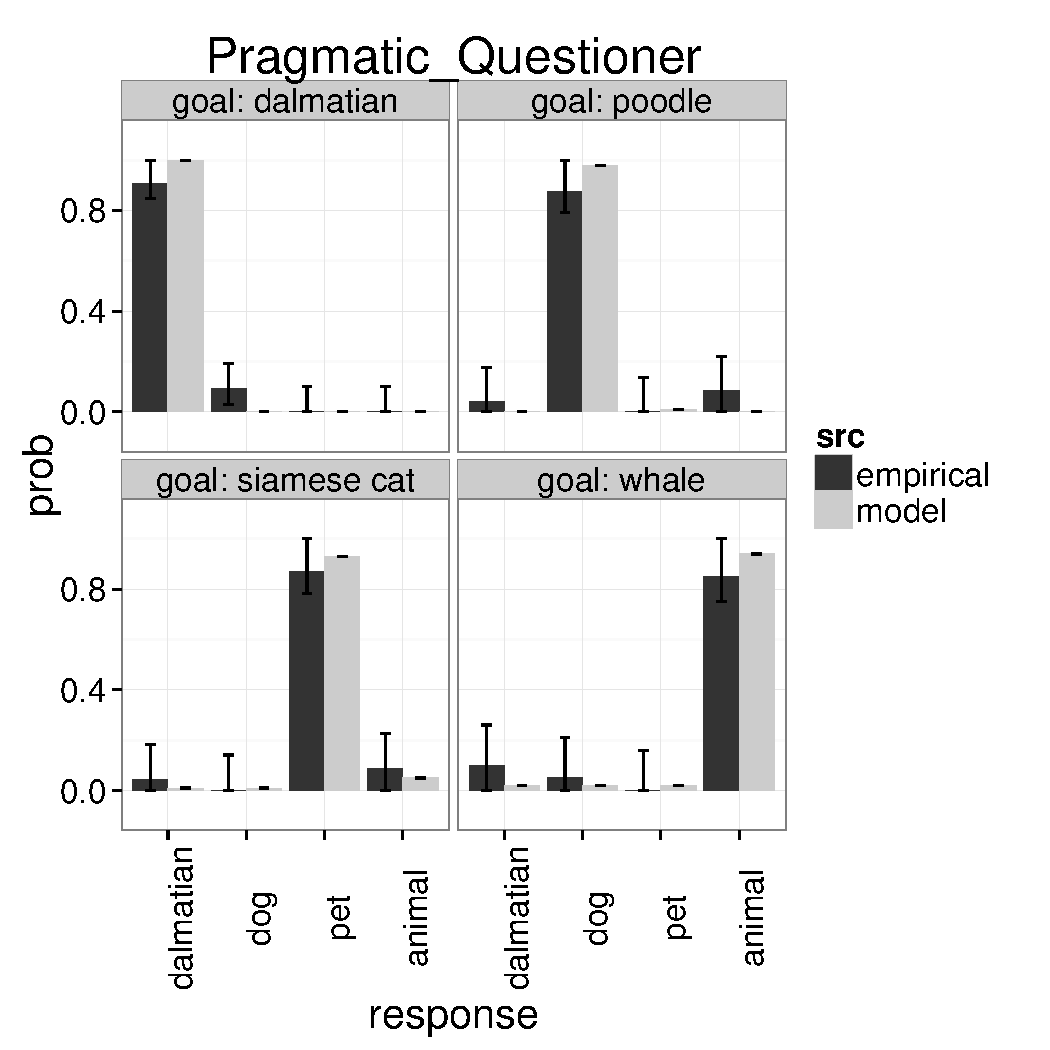
\includegraphics[scale = .4]{Exp3PragmaticQuestioner.pdf}
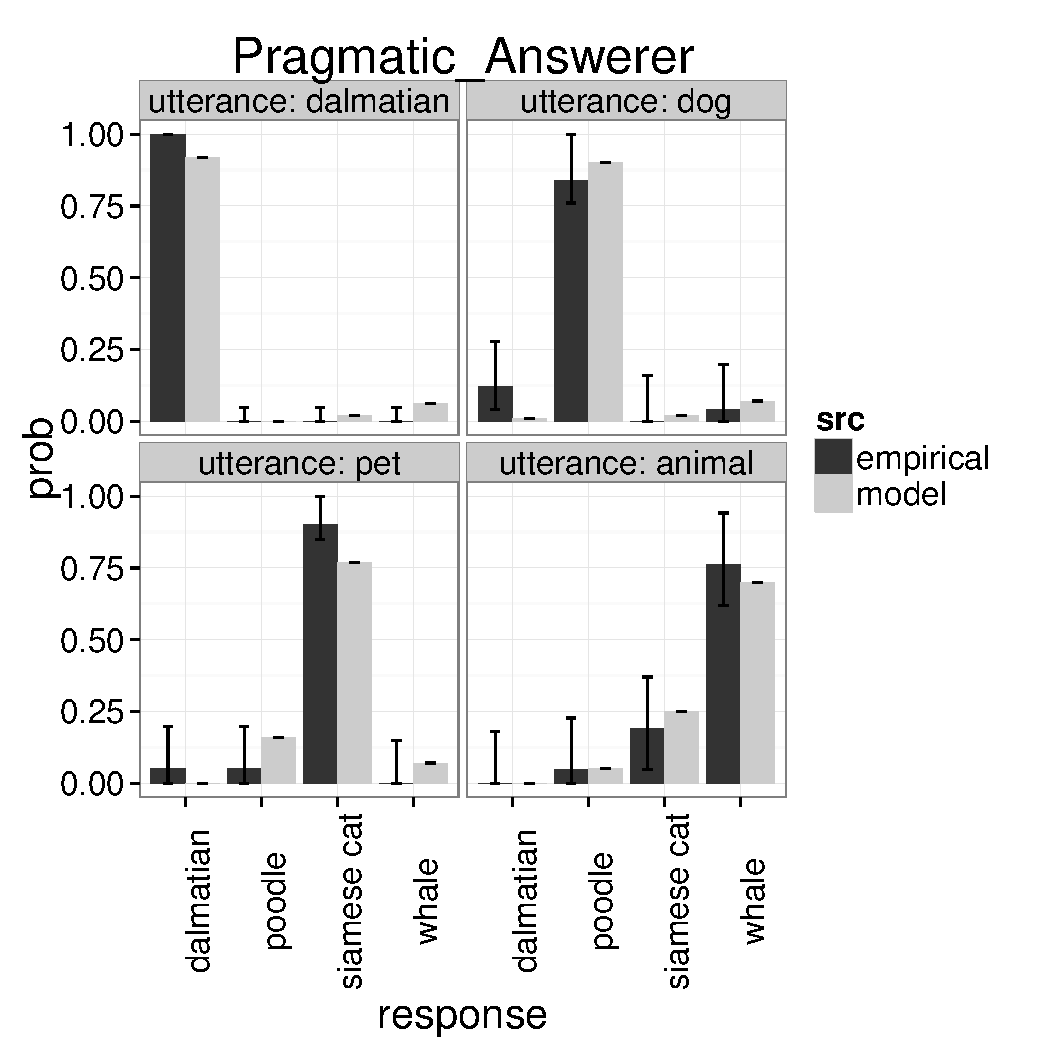
\includegraphics[scale = .4]{Exp3PragmaticAnswerer.pdf}
\end{center}
\vspace{-.5cm}
\caption{Exp.~3 results and model fits, for the best-performing questioenr (left) and answerer (right) models.}
\vspace{-.1cm}
\label{fig:exp3res}
\end{figure}

\subsubsection{Model comparison}

Model comparison was conducted in the same way as in Experiment 1: a single optimality parameter, which applied to all agents, was fit for each of the six models to maximize correlation with the data.

We can again rule out both the literal answerer and literal questioner as they predict a uniform distribution of responses over the four questions and answers. The two remaining questioner models again make roughly the same predictions for this task:
we found a model-data correlation of $r = 0.971$ for the explicit questioner and correlation of $r = 0.996$ for the pragmatic questioner. The difference between these correlations is statistically significant, accounting for their shared dependence on the empirical data (Zou's confidence interval $= [-0.079, -0.009]$). However, they make nearly identical qualitative predictions; the pragmatic questioner model's predictions for each response distribution are shown in Fig.~\ref{fig:exp3res} (left). 

The pragmatic answerer provides a much better fit to the data than the explicit answerer: we find a model-data correlation of $r = 0.7$ for the explicit answerer and $r = 0.99$ for the pragmatic answerer.  Taking into account the fact that these correlations are dependent and overlapping on the same empirical data, we find that the pragmatic answerer correlation is significantly larger than the explicit answerer correlation (Zou's confidence interval $= [-0.676, -0.107]$). 
%
\begin{figure}[t!]
\begin{center}
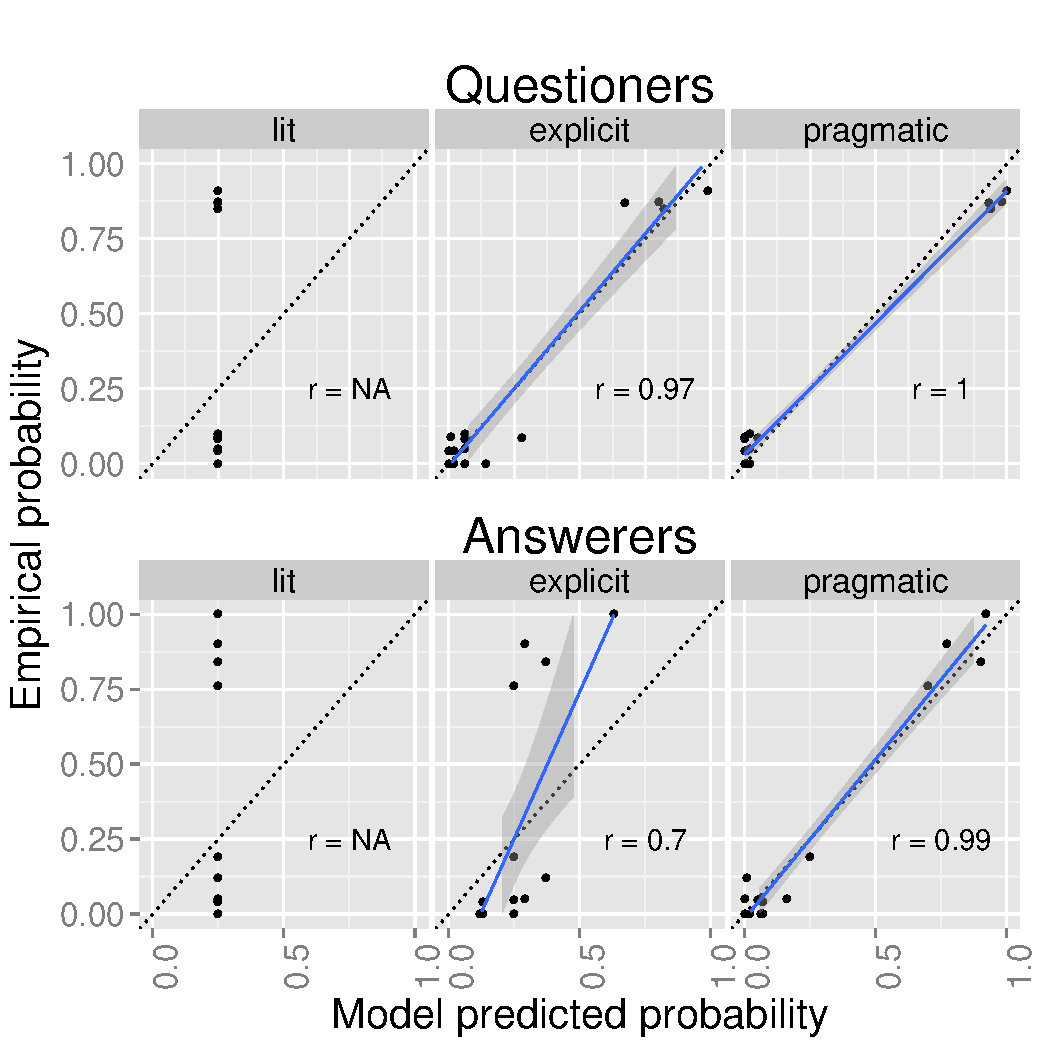
\includegraphics[scale=.75]{Exp3ModelFits.pdf}
\end{center}
\vspace{-.5cm}
\caption{Full space of models, and their correlations with the data from Exp.~1. Questioner models in the first row reason about the answerers directly below them, and the pragmatic answerer reasons about the explicit questioner.}
\label{fig:Exp3ModelSpace}
\vspace{-.15cm}
\end{figure}
%

\subsubsection{Discussion}

We replicated the results of experiment 1 in a real-time, interactive setting. Again, we found that both explicit and pragmatic questioner models provide an excellent fit to questioner behavior, and that the pragmatic answerer accounts for the data significantly better than the explicit answerer both quantitatively and qualitatively. In addition, the full, interactive game was designed to be more natural and less confusing to participants than the drop-down menu design from experiments 1 and 2. Because players received constant feedback from their partner, this task was framed as inherently social, and because answerers watched as questioners moved words to form questions, there was a convincing mechanism for people to believe they were playing with another human. This addresses some concerns raised with experiments 1 and 2. 

Note that so far we have used the same animal hierarchy for the stimulus set in all our experiments, providing only 16 points of comparison between our models and empirical data. Furthermore, there exists a heuristic strategy for selecting questions given goals in the hierarchy structure we have been using which produces the same pattern of responses without requiring any social inference. Suppose questioners saw their goal on a given trial and ruled out labels that do not apply (e.g. a `cat' is neither a `dalmatian' nor a `dog'), then picked the most specific of the remaining labels (`pet' picks out a smaller set of objects than `animal').  
 
In experiment 4, we test the generality of our model by expanding the stimulus set to encompass multiple stimulus domains and multiple hierarchy structures. This addresses the potential concern that the behavioral patterns we have been modeling are specific to the set of animals we decided to use or the tree-like hierarchy in which they were embedded. We also took care to include one simple but critical hierarchy structure where (1) the explicit and pragmatic questioner models make different predictions and (2) the heuristic strategy cannot explain these predictions. 


\section{General discussion}
\label{sec:gd}

Perhaps the most important formal advance of the models considered here is to move the Rational Speech Act framework beyond interpretation of single utterances (in context), to consider the dynamics of simple dialogs (albeit consisting of a single question and its answer). 
Doing so requires replacing the immediate motive to convey true information with the more distant motive to provoke useful information from one's interlocutor. On the answerer side, sophisticated inference was required to account for the implicit interests of the questioner. This provides a useful connection to current game-theoretic and decision-theoretic models \cite{VogelBodoiaPottsJurafsky13_GricePOMDP, VanRooy03_QuestioningDecisionProblems}, which also emphasize the importance of goals and speaker beliefs in communication but emphasize less the complex interplay of inference between questioner and answerer.

We have presented evidence that answerer behavior is best described by a pragmatic model that \emph{does} reason about questioner intentions, using the question utterance as a signal. The superiority of pragmatic answerer predictions over the other answerer models was robust. Questioner behavior in Exp.~2, however, seemed to be much more dependent on experience. 
In another version of Exp.~1, we did not emphasize certain aspects of the game in the instructions, such as the fact that the answerer knows about the restricted answer set, which might prompt perspective-taking. 
Our data in this pilot experiment appeared to contain a mixture of explicit and pragmatic answerers and questioners (though other confounds were present in this version).
%These instructions reflect essential assumptions of the model and without these instructions, questioner behavior shifted more toward that predicted by the explicit model. 
%Indeed, it appears that our sample contained a mixture of explicit and pragmatic questioners. 
Overall, it will be important to explore the mixture of explicit- and pragmatic-questioning across a larger range of situations:
these issues may be a product of our artificial game paradigm, or they may be reflective of real tendencies in language use, raising novel questions about audience design in question-answer behavior.


While the artificiality of our question-answer game may distance the behavior of participants from the natural use of language, there are also some benefits to this design. In particular, it is easy in this setting to control the exact space of questions, goals, and answers. While the restrictions on question space may seem peculiar, it is directly motivated by conversational scenarios in everyday usage which feature restrictions on the set of things one can ask about, due to politeness, salience, time cost, and other factors. In future work, we will explore the extent to which the proposed model can scale up to real-time, multiplayer games, extended dialogues, and other more naturalistic language settings. To deal with dialogues lasting longer than a single exchange, for instance, we must specify the way in which the contributions of questioner and answerer affect the \emph{context} in which later utterances operate.

Humans are experts at inferring the intentions of other agents from their actions \cite{TomaselloCarpenter___Moll05_IntentionsCulturalCognition}. Given simple motion cues, for example, we are able to reliably discern high-level goals such as chasing, fighting, courting, or playing \cite{BarrettToddMillerBlythe05_IntentionFromMotionCues, HeiderSimmel44_Animacy}. Experiments in psycholinguistics have shown that this expertise extends to speech acts.  Behind every question lies a goal or intention. This could be an intention to obtain an explicit piece of information (``Where can I get a newspaper?''), signal some common ground (``Did you see the game last night?''), test the answerer's knowledge (``If I add these numbers together, what do I get?''), politely request the audience to take some action (``Could you pass the salt?''), or just to make open-ended small talk (``How was your weekend?''). These wildly different intentions seem to warrant different kinds of answers%, even if the explicit question is expressed using the same words
. By formalizing the computational process by which answerers infer these different intentions, our model framework provides a unifying way to accommodate this diversity.  % If questions themselves are informative, we must ask them carefully.


\bibliography{fyp}
\bibliographystyle{apacite}


\end{document}  
